\chapter{Simple Modules}
\label{cha:simple-modules}
\index{module!simple}


\textit{Simple modules} are the active components in the model.
Simple modules are programmed in C++, using the {\opp} class
library. The following sections contain a short introduction
to discrete event simulation in general, explain how its concepts are
implemented in {\opp}, and give an overview and practical advice
on how to design and code simple modules.



\section{Simulation concepts}

This section contains a very brief introduction into how Discrete
Event Simulation (DES) works, in order to introduce terms we'll use
when explaining {\opp} concepts\index{simulation!concepts} and
implementation.


\subsection{Discrete Event Simulation}

A \textit{Discrete Event System} is a system where state changes
(events\index{events}) happen at discrete instances in time, and events take zero time
to happen. It is assumed that nothing (i.e. nothing interesting)
happens between two consecutive events, that is, no state change takes
place in the system between the events (in contrast to
\textit{continuous} systems where state changes are continuous). Those
systems that can be viewed as Discrete Event Systems can be modeled
using Discrete Event Simulation\index{discrete event simulation}.
(Other systems can be modelled e.g. with continuous simulation models.)

For example, computer networks are usually viewed as discrete
event systems. Some of the events are:

\begin{itemize}
  \item{start of a packet transmission}
  \item{end of a packet transmission}
  \item{expiry of a retransmission timeout}
\end{itemize}


This implies that between two events such as \textit{start of a packet
transmission} and \textit{end of a packet transmission}, nothing
interesting happens. That is, the packet's state remains \textit{being
transmitted}. Note that the definition of ``interesting'' events and states always
depends on the intent and purposes of the person doing the modeling.
If we were interested in the transmission of individual bits, we would
have included something like \textit{start of bit transmission} and
\textit{end of bit transmission} among our events.


The time when events occur is often called \textit{event timestamp}
\index{event timestamp}; with {\opp} we'll say
\textit{arrival time}\index{arrival time} (because in the class
library, the word ``timestamp'' is reserved for a user-settable
attribute in the event class). Time within the model is often called
\textit{simulation time}\index{simulation time}, \textit{model time}
\index{model!time} or \textit{virtual time}\index{virtual time}
as opposed to real time\index{real time} or CPU time\index{CPU time}
which refer to how long the simulation program has been running and
how much CPU time it has consumed.



\subsection{The event loop}

Discrete event simulation maintains the set of future
events\index{future events} in a data structure often called
FES\index{FES} (Future Event Set) or FEL\index{FEL} (Future Event List).
Such simulators usually work according to the following pseudocode:

\begin{Verbatim}[commandchars=\\\{\}]
\textit{initialize -- this includes building the model and}
              \textit{inserting initial events to FES}

\textit{while (FES not empty and simulation not yet complete)}
\textit{\{}
    \textit{retrieve first event from FES}
    \textit{t:= timestamp of this event}
    \textbf{\textit{process event}}
    \textit{(processing may insert new events in FES or delete existing ones)}
\textit{\}}
\textit{finish simulation (write statistical results, etc.)}
\end{Verbatim}


The first, initialization step usually builds the data structures
representing the simulation model, calls any user-defined
initialization code, and inserts initial events\index{initial events}
into the FES\index{FES} to ensure that the simulation can start. Initialization
strategy can differ considerably from one simulator to another.


The subsequent loop consumes events from the FES\index{FES} and processes
them. Events are processed in strict timestamp order in order
to maintain causality, that is, to ensure that no event may have
an effect on earlier events.

Processing an event involves calls to user-supplied code. For example,
using the computer network simulation example, processing a ``timeout
expired'' event may consist of re-sending a copy of the network
packet, updating the retry count, scheduling another ``timeout''
event, and so on. The user code may also remove events from the FES\index{FES},
for example when canceling timeouts.

The simulation stops when there are no events left (this happens
rarely in practice), or when it isn't necessary for the simulation
to run further because the model time or the CPU time has reached
a given limit, or because the statistics have reached the desired
accuracy. At this time, before the program exits, the user
will typically want to record statistics into output files.



\subsection{Simple modules in {\opp}}
\label{sec:simple-modules-in-opp}

In {\opp}, events occur inside simple modules\index{module!simple}.
Simple modules encapsulate C++ code that generates events and reacts to events,
in other words, implements the behaviour of the model.

The user creates simple module types by subclassing the \cclass{cSimpleModule}
class, which is part of the {\opp} class library.
\cclass{cSimpleModule}, just as \cclass{cCompoundModule}, is derived
from a common base class, \cclass{cModule}.

\cclass{cSimpleModule}, although packed with simulation-related
functionality, doesn't do anything useful by itself -- you have
to redefine some virtual member functions to make it do useful work.


These member functions are the following:
\begin{itemize}
  \item{void \fname{initialize()}}
  \item{void \fname[handleMessage()]{handleMessage(cMessage *msg)}}
  \item{void \fname{activity()}}
  \item{void \fname{finish()}}
\end{itemize}

In the initialization step, {\opp} builds the network: it creates the
necessary simple\index{module!simple} and compound modules and
connects them according to the NED definitions. {\opp} also calls the
\fname{initialize()} functions of all modules.

The \fname{handleMessage()} and \fname{activity()} functions are
called during event processing. This means that the user will
implement the model's behavior in these functions.
\fname{handleMessage()} and \fname{activity()} implement
different event processing strategies: for each simple module, the user
has to redefine exactly one of these functions.

\fname{handleMessage()} is a method that is called
by the simulation kernel when the module receives a message.
\fname{activity()} is a coroutine-based\index{coroutine} solution
which implements the process interaction approach (coroutines are
non-preemptive (i.e. cooperative) threads). Generally, it is recommended
that you prefer \fname{handleMessage()} to \fname{activity()} --
mainly because \fname{activity()} doesn't scale well.
Later in this chapter we'll discuss both methods including their advantages
and disadvantages.

Modules written with \fname{activity()} and \fname{handleMessage()}
can be freely mixed within a simulation model.

The \fname{finish()} functions are called when the simulation
terminates successfully. The most typical use of \fname{finish()}
is the recording of statistics collected during simulation.



\subsection{Events in {\opp}}

{\opp} uses messages\index{message} to represent
events\index{events}. Each event is represented by an instance of the
\cclass{cMessage} class or one its subclasses; there is no separate
event class. Messages are sent from one module to another -- this
means that the place where the ``event will occur'' is the
\textit{message's destination module}, and the model time when the
event occurs is the \textit{arrival time}\index{arrival time} of the
message. Events like ``timeout expired'' are implemented by the
module sending a message to itself.

Events are consumed from the FES\index{FES} in arrival time order, to
maintain causality. More precisely, given two messages, the following
rules apply:
\begin{enumerate}
\item{the message with \textbf{earlier arrival time} is executed
    first.  If arrival times are equal,}
\item{the one with \textbf{smaller priority value} is executed first.
    If priorities are the same,}
\item{the one \textbf{scheduled or sent earlier} is executed first.}
\end{enumerate}

\textit{Priority}\index{message!priority} is a user-assigned integer
attribute of messages.

\subsection{Simulation time}

The current simulation time can be obtained with the \ttt{simTime()} function.

Simulation time in {\opp} is represented by the C++ type \fvar{simtime\_t},
which is by default a typedef to the \ttt{SimTime} class.
\ttt{SimTime} class stores simulation time in a 64-bit integer,
using decimal fixed-point representation. The resolution is controlled
by the \textit{scale exponent} global configuration variable, that is,
\ttt{SimTime} instances have the same resolution. The exponent can be
between chosen between -18 (attosecond resolution) and 0 (seconds).
Some exponents with the ranges they provide are shown in the following table.

\begin{center}
  \begin{tabular}{ | r | r | c | }
    \hline
    Exponent & Resolution & Approx. Range \\ \hline
     -18 & $10^{-18}$s (1as) & $\pm 9.22$s \\
     -15 & $10^{-15}$s (1fs) & $\pm 153.72$ minutes \\
     -12 & $10^{-12}$s (1ps) & $\pm 106.75$ days \\
     -9  & $10^{-9}$s (1ns)  & $\pm 292.27$ years \\
     -6  & $10^{-6}$s (1us)  & $\pm 292271$ years \\
     -3  & $10^{-3}$s (1ms)  & $\pm 2.9227e8$ years \\
     0   & 1s                & $\pm 2.9227e11$ years \\
    \hline
  \end{tabular}
\end{center}

Note that although simulation time cannot be negative, it is still useful to
be able to represent negative numbers, because they often arise
during the evaluation of arithmetic expressions.

The \ttt{SimTime} class performs additions and substractions as 64-bit integer
operations. Integer overflows are checked, and will cause the simulation to
stop with an error message. Other operations (multiplication, division, etc)
are performed in \ttt{double}, then converted back to integer.

There is no implicit conversion from \ttt{SimTime} to \ttt{double}, mostly
because it would conflict with overloaded arithmetic operations of \ttt{SimTime};
use the \fname{dbl()} method of \ttt{Simtime} to convert. To reduce the
need for \fname{dbl()}, several functions and methods have overloaded variants
that directly accept \ttt{SimTime}, for example \fname{fabs()}, \fname{fmod()},
\fname{ceil()}, \fname{floor()}, \fname{uniform()}, \fname{exponential()}, and
\fname{normal()}.

\begin{note}
   Converting a \ttt{SimTime} to \ttt{double} may lose precision, because
   \ttt{double} has only a 52-bit mantissa.
\end{note}

Other useful methods of \ttt{SimTime} include \fname{str()}
which returns the value as a string; \fname{parse()} which converts a
string to \ttt{SimTime}; \fname{raw()} which returns the
underlying \ttt{int64} value; \fname{getScaleExp()} which returns the
global scale exponent; and \fname{getMaxTime} which returns the
maximum simulation time that can be represented at the current
scale exponent.

Earlier versions of \opp used \ttt{double} for simulation time. To facilitate
porting existing models to \opp 4.0 or later, \opp can be compiled to use
\ttt{double} for \ttt{simtime\_t}. To enable this mode, define the
\ttt{USE\_DOUBLE\_SIMTIME} preprocessor macro during compiling \opp
and the simulation models. There are also several macros that can be used
in simulation models to make them compile with both \ttt{simtime\_t}'s:
\fmac{SIMTIME\_STR()} which converts simulation time to a \ttt{const char *}
(this macro can be used inside \ttt{printf}'s);
\fmac{SIMTIME\_DBL(t)} which converts simulation time to \ttt{double};
\fmac{SIMTIME\_RAW(t)} which returns the underlying \ttt{int64} or \ttt{double};
\fmac{STR\_SIMTIME(s)} which converts string to simulation time; and
\fmac{SIMTIME\_TTOA(buf,t)} which converts simulation time to string,
and places the result into the given buffer. \fmac{MAXTIME} is
also defined correctly for both \ttt{simtime\_t} types.

\begin{note}
   Why did \opp switch to \ttt{int64}-based simulation time?
   \ttt{double}'s mantissa is only 52 bits long, and this caused
   problems in long simulations that relied on fine-grained timing,
   for example MAC protocols. Other problems were the accumulation of
   rounding errors, and non-associativity (often $(x+y)+z \neq x+(y+z)$, see
   ~\cite{Goldberg91what}) which meant that two \ttt{double} simulation
   times could not be reliably compared for equality.
\end{note}


\subsection{FES implementation}

The implementation of the FES\index{FES} is a crucial factor in the
performance of a discrete event simulator. In {\opp}, the FES is
implemented with \textit{binary heap}\index{binary heap}, the most
widely used data structure for this purpose. Heap is also the best
algorithm we know, although exotic data structures like
\textit{skiplist}\index{skiplist} may perform better than heap in some
cases. In case you're interested, the FES implementation is in the
\cclass{cMessageHeap} class, but as a simulation programmer you won't
ever need to care about that.





\section{Defining simple module types}

\subsection{Overview}

As mentioned before \ref{sec:simple-modules-in-opp}, a simple module\index{module!simple}
is nothing more than a C++ class which has to be subclassed from
\cclass{cSimpleModule}, with one or more virtual member functions redefined
to define its behavior.

The class has to be registered with {\opp} via the \fmac{Define\_Module()} macro.
The \fmac{Define\_Module()} line should always be put into \ttt{.cc} or \ttt{.cpp}
files and not header file (\ttt{.h}), because the compiler generates code from it.
      \footnote{For completeness, there is also a \fmac{Define\_Module\_Like()}
                macro, but its use is discouraged and might even be removed in
                future {\opp} releases.}

The following \ttt{HelloModule} is about the simplest simple module one could write.
(We could have left out the \ttt{initialize()} method as well to make it even smaller,
but how would it say Hello then?) Note \cclass{cSimpleModule} as base class,
and the \fmac{Define\_Module()} line.

\begin{verbatim}
// file: HelloModule.cc
#include <omnetpp.h>

class HelloModule : public cSimpleModule
{
  protected:
    virtual void initialize();
    virtual void handleMessage(cMessage *msg);
};

// register module class with OMNeT++
Define_Module(HelloModule);

void HelloModule::initialize()
{
    ev << "Hello World!\n";
}

void HelloModule::handleMessage(cMessage *msg)
{
    delete msg; // just discard everything we receive
}
\end{verbatim}

In order to be able to refer to this simple\index{module!simple} module type
in NED files, we also need an associated NED declaration which might
look like this:

\begin{Verbatim}[commandchars=\\\{\}]
// file: HelloModule.ned
\textbf{simple} HelloModule
    \textbf{gates}:
        \textbf{in:} in;
\textbf{endsimple}
\end{Verbatim}


\subsection{Constructor}

Simple modules are never instantiated by the user directly, but rather by
the simulation kernel. This implies that one cannot write arbitrary
constructors: the signature must be what is expected by the simulation kernel.
Luckily, this contract is very simple: the constructor must be public, and must take
no arguments:

\begin{verbatim}
  public:
    HelloModule();  // constructor takes no arguments
\end{verbatim}

\cclass{cSimpleModule} itself has two constructors:
\begin{enumerate}
  \item{\ttt{cSimpleModule()} -- one without arguments}
  \item{\ttt{cSimpleModule(size\_t stacksize)} -- one that accepts the coroutine
        stack size\index{module!stack size}\index{stack!size}}
\end{enumerate}

The first version should be used with \fname{handleMessage()} simple modules,
and the second one with \fname{activity()} modules.
(With the latter, the \fname{activity()} method of the module class
runs as a coroutine\index{coroutine} which needs a separate CPU stack,
usually of 16..32K. This will be discussed in detail later.)
Passing zero stack size to the latter constructor also selects \ttt{handleMessage()}.

Thus, the following constructor definitions are all OK, and select
\fname{handleMessage()} to be used with the module:

\begin{verbatim}
HelloModule::HelloModule() {...}
HelloModule::HelloModule() : cSimpleModule() {...}
\end{verbatim}

It is also OK to omit the constructor altogether, because the
compiler-generated one is suitable too.

The following constructor definition selects \fname{activity()} to be used
with the module, with 16K of coroutine stack:

\begin{verbatim}
HelloModule::HelloModule() : cSimpleModule(16384) {...}
\end{verbatim}

\begin{note}
    The \fmac{Module\_Class\_Members()} macro, already deprecated in \opp 3.2,
    has been removed in the 4.0 version. When porting older simulation models,
    occurrences of this macro can simply be removed from the source code.
\end{note}



\subsection{Constructor and destructor vs initialize() and finish()}

The \fname{initialize()} and \fname{finish()} methods will be discussed
in a later section in detail, but because their apparent similarity
to the constructor and the destructor is prone to cause some confusion,
we'll briefly cover them here.

The constructor gets called when the module is created, as part of the
model setup process. At that time, everything is just being built,
so there isn't a lot things one can do from the constructor.
In contrast, \fname{initialize()} gets called just before the
simulation starts executing, when everything else has been set up
already.

\fname{finish()} is for recording statistics, and it only gets called
when the simulation has terminated normally. It does not get called when
the simulations stops with an error message. The destructor always
gets called at the end, no matter how the simulation stopped, but
at that time it is fair to assume that the simulation model has been
halfway demolished already.

Based on the above, the following conventions exist for these four methods:

\begin{description}

\item Constructor:

Set pointer members of the module class to \ttt{NULL}; postpone all other
initialization tasks to \fname{initialize()}.

\item \fname{initialize()}:

Perform all initialization tasks: read module parameters, initialize
class variables, allocate dynamic data structures with \ttt{new};
also allocate and initialize self-messages (timers) if needed.

\item \fname{finish()}:

Record statistics. Do \tbf{not} \ttt{delete} anything or cancel timers --
all cleanup must be done in the destructor.

\item Destructor:

Delete everything which was allocated by \ttt{new} and is still held
by the module class. With self-messages (timers), use the
\fname{cancelAndDelete(msg)} function! It is almost always wrong
to just delete a self-message from the destructor, because it might be
in the scheduled events list. The \fname{cancelAndDelete(msg)} function
checks for that first, and cancels the message before deletion if necessary.

\end{description}


\subsection{"Garbage collection" and compatibility}
\label{sec:garbage-collection}

{\opp} versions before the 3.2 release had a feature which often was,
informally and also somewhat incorrectly, called \textit{"garbage
collection"} (GC). The purpose of this feature was to mitigate the need for
writing destructors, and often constructors as well by providing automatic
cleanup at the end of the simulation. (It did not do anything during
simulation, as the name might suggest.)

{\opp} (all versions) keep track of user-allocated simulation objects
(typically: messages) and their ownerships. What the \textit{"garbage
collection"} feature did was that during the cleanup of the model, after
each module destructor finished, it checked whether there were simulations
objects left that were apparently owned by that module but not deallocated
by the destructor -- and if it found such objects, it invoked \ttt{delete}
on them.

It worked out nicely in 90 percent of cases, but occasionally it resulted
in spurious crashes which were hard to debug for users not familiar
with {\opp} internals or lacking advanced C++ skills.
    \footnote{These crashes occurred due to lack of information available
              to the GC mechanism, e.g. C++ provides no way to detect
              from the pointer whether an object is part of an array, or is
              inside a struct or class. The solution was to use pointers:
              pointer array, pointer as class member, etc.}

Starting from {\opp} 3.2, this cleanup-time GC mechanism has been disabled by default
(\ttt{perform-gc=} configuration option, see \ref{sec:ch-run-sim:general-section}),
and it generally not recommended to turn it back on. It does not do any harm
to run any simulation model without GC (apart from the memory leak).

It is expected that existing modules will be updated sooner or later, by adding
proper constructors and destructors. To catalyse this process, {\opp} dumps the
list of unreleased objects at the end of the simulation. This dump can also be
turned off in the configuration (\ttt{print-undisposed=} configuration option,
see \ref{sec:ch-run-sim:general-section}).



\subsection{An example}

The following code is a bit longer but actually useful simple module
implementation. It demonstrates several of the above concepts, plus
some others which will be explained in later sections:
\begin{enumerate}
  \item{constructor, initialize and destructor conventions}
  \item{using messages for timers}
  \item{accessing module parameters}
  \item{recording statistics at the end of the simulation}
  \item{documenting the programmer's assumptions using ASSERT()}
\end{enumerate}

\begin{verbatim}
// file: FFGenerator.h

#include <omnetpp.h>

/**
 * Generates messages or jobs; see NED file for more info.
 */
class FFGenerator : public cSimpleModule
{
  private:
    cMessage *sendMessageEvent;
    long numSent;

  public:
    FFGenerator();
    virtual ~FFGenerator();

  protected:
    virtual void initialize();
    virtual void handleMessage(cMessage *msg);
    virtual void finish();
};
\end{verbatim}

\begin{verbatim}
// file: FFGenerator.cc

#include "FFGenerator.cc"

// register module class with OMNeT++
Define_Module(FFGenerator);

FFGenerator::FFGenerator()
{
    sendMessageEvent = NULL;
}

void FFGenerator::initialize()
{
    numSent = 0;
    sendMessageEvent = new cMessage("sendMessageEvent");
    scheduleAt(0.0, sendMessageEvent);
}

void FFGenerator::handleMessage(cMessage *msg)
{
    ASSERT(msg==sendMessageEvent);

    cMessage *m = new cMessage("packet");
    m->setBitLength(par("msgLength"));
    send(m, "out");
    numSent++;

    double deltaT = (double)par("sendIaTime");
    scheduleAt(simTime()+deltaT, sendMessageEvent);
}

void FFGenerator::finish()
{
    recordScalar("packets sent", numSent);
}

FFGenerator::~FFGenerator()
{
    cancelAndDelete(sendMessageEvent);
}
\end{verbatim}

The corresponding NED declaration:

\begin{Verbatim}[commandchars=\\\{\}]
// file: FFGenerator.ned
\textbf{simple} FFGenerator
\{
    \textbf{parameters}:
        \textbf{volatile double} sendIaTime;
    \textbf{gates}:
        \textbf{output} out;
\}
\end{Verbatim}




\subsection{Using global variables}
\index{global variables}

If possible, avoid using global variables, including
static class members. They are prone to cause several problems.
First, they are not reset to their initial values (to zero)
when you rebuild the simulation in Tkenv, or start another run
in Cmdenv. This may produce surprising results.
Second, they prevent you from running your simulation in parallel.
When using parallel simulation, each partition of your model
(may) run in a separate process, having its own copy of the
global variables. This is usually not what you want.

The solution is to encapsulate the variables into simple modules
as private or protected data members, and expose them via public methods.
Other modules can then call these public methods to get or set the values.
Calling methods of other modules will be discussed in section
\ref{ch:simple-modules:direct-method-calls}.
Examples of such modules are the \ttt{Blackboard} in the \textit{Mobility Framework},
and \ttt{InterfaceTable} and \ttt{RoutingTable} in the \textit{INET Framework}.



\section{Adding functionality to cSimpleModule}

This section discusses \cclass{cSimpleModule}'s four previously
mentioned member functions, intended to be redefined by the user:
\fname{initialize()}, \fname{handleMessage()}, \fname{activity()}
and \fname{finish()}, plus a fifth, less frequently used one,
\fname{handleParameterChange}.



\subsection{handleMessage()}

\subsubsection{Function called for each event}


The idea is that at each event\index{event} (message arrival) we
simply call a user-defined function. This function,
\ttt{handleMessage(cMessage *msg)} is a
virtual member function of \cclass{cSimpleModule} which does
nothing by default -- the user has to redefine it in subclasses
and add the message processing code.

The \fname{handleMessage()} function will be called for every message
that arrives at the module. The function should process the message
and return immediately after that. The simulation time is potentially
different in each call. No simulation time elapses within a call
to \fname{handleMessage()}.

The event loop inside the simulator handles both \fname{activity()}
and \fname{handleMessage()} simple modules, and it corresponds
to the following pseudocode:

\begin{Verbatim}[commandchars=\\\{\}]
\textit{while (FES not empty and simulation not yet complete)}
\{
    retrieve first event from FES
    t:= timestamp of this event
    m:= module containing this event
    if (m works with handleMessage())
        \textbf{m->handleMessage( event )}
    else // m works with activity()
        transferTo( m )
\}
\end{Verbatim}

Modules with \fname{handleMessage()} are NOT started automatically:
the simulation kernel creates starter messages\index{starter messages}
only for modules with \fname{activity()}. This means that you have to
schedule self-messages\index{self-message} from the
\fname{initialize()} function if you want a \fname{handleMessage()}
simple module to start working ``by itself'', without first receiving
a message from other modules.


\subsubsection{Programming with handleMessage()}


To use the \fname{handleMessage()} mechanism in a
simple module, you must specify \textit{zero
  stack size}\index{zero stack size} for the module. This is
important, because this tells {\opp} that you want to use
\fname{handleMessage()} and not \fname{activity()}.

Message/event related functions you can use in \fname{handleMessage()}:

\begin{itemize}
  \item{\fname{send()} family of functions -- to send messages to other modules}
  \item{\fname{scheduleAt()} -- to schedule an event (the module ``sends a message to itself'')}
  \item{\fname{cancelEvent()} -- to delete an event scheduled with \fname{scheduleAt()}}
\end{itemize}

You cannot use the \fname{receive()} family and
\fname{wait()} functions in \fname{handleMessage()}, because they are
coroutine-based by nature, as explained in the section about
\fname{activity()}.

You have to add data members to the module class for every piece
of information you want to preserve. This information cannot
be stored in local variables of \fname{handleMessage()} because they
are destroyed when the function returns. Also, they cannot be
stored in static variables in the function (or the class), because
they would be shared between all instances of the class.


Data members to be added to the module class will typically include
things like:

\begin{itemize}
  \item{state (e.g. IDLE/BUSY, CONN\_DOWN/CONN\_ALIVE/...)}
  \item{other variables which belong to the state of the module: retry
    counts, packet queues, etc.}
  \item{values retrieved/computed once and then stored: values of module
    parameters, gate indices, routing information, etc.}
  \item{pointers of message objects created once and then reused for
    timers, timeouts, etc.}
  \item{variables/objects for statistics collection}
\end{itemize}

You can initialize these variables from the \fname{initialize()}
function.  The constructor\index{module!constructor} is not a very good place
for this purpose, because it is called in the network setup phase when
the model is still under construction, so a lot of information you may
want to use is not yet available.

Another task you have to do in \fname{initialize()} is to schedule
initial event(s)\index{events!initial} which trigger the first call(s)
to \fname{handleMessage()}.  After the first call,
\fname{handleMessage()} must take care to schedule further events for
itself so that the ``chain'' is not broken. Scheduling events is not
necessary if your module only has to react to messages coming from
other modules.

\fname{finish()} is normally used to record statistics information
accumulated in data members of the class at the end of the simulation.


\subsubsection{Application area}


\fname{handleMessage()} is in most cases a better choice than \fname{activity()}:

\begin{enumerate}
  \item{When you expect the module to be used in large simulations,
      involving several thousand modules. In such cases, the module stacks
      required by \fname{activity()} would simply consume too much memory.}
  \item{For modules which maintain little or no state information,
      such as packet sinks, \fname{handleMessage()} is more convenient to program.}
  \item{Other good candidates are modules with a large state space and
      many arbitrary state transition possibilities (i.e. where there
      are many possible subsequent states for any state). Such algorithms
      are difficult to program with \fname{activity()}, or the result is code
      which is better suited for \fname{handleMessage()} (see rule of thumb
      below). Most communication protocols are like this.}
\end{enumerate}


\subsubsection{Example 1: Protocol models}

Models of protocol layers in a communication network tend to have
a common structure on a high level because fundamentally they all have to react
to three types of events: to messages arriving from higher layer protocols
(or apps), to messages arriving from lower layer protocols (from the network),
and to various timers and timeouts (that is, self-messages).

This usually results in the following source code pattern:

\begin{verbatim}
class FooProtocol : public cSimpleModule
{
  protected:
    // state variables
    // ...

    virtual void processMsgFromHigherLayer(cMessage *packet);
    virtual void processMsgFromLowerLayer(FooPacket *packet);
    virtual void processTimer(cMessage *timer);

    virtual void initialize();
    virtual void handleMessage(cMessage *msg);
};

// ...

void FooProtocol::handleMessage(cMessage *msg)
{
    if (msg->isSelfMessage())
        processTimer(msg);
    else if (msg->arrivedOn("fromNetw"))
        processMsgFromLowerLayer(check_and_cast<FooPacket *>(msg));
    else
        processMsgFromHigherLayer(msg);
}
\end{verbatim}

The functions \ttt{processMsgFromHigherLayer()}, \ttt{processMsgFromLowerLayer()}
and \ttt{processTimer()} are then usually split further: there are separate
methods to process separate packet types and separate timers.


\subsubsection{Example 2: Simple traffic generators and sinks}


The code for simple packet generators and sinks programmed with \fname{handleMessage()} might
be as simple as the following pseoudocode:

\begin{verbatim}
PacketGenerator::handleMessage(msg)
{
    create and send out a new packet;
    schedule msg again to trigger next call to handleMessage;
}

PacketSink::handleMessage(msg)
{
    delete msg;
}
\end{verbatim}

Note that \textit{PacketGenerator} will need to redefine \fname{initialize()}
to create \textit{m} and schedule the first event.

The following simple module generates packets with exponential
inter-arrival time. (Some details in the source haven't been
discussed yet, but the code is probably understandable nevertheless.)


\begin{Verbatim}[commandchars=\\\{\}]
class Generator : public cSimpleModule
\{
  public:
    Generator() : cSimpleModule() {}
  protected:
    virtual void initialize();
    virtual void handleMessage(cMessage *msg);
\};

Define_Module(Generator);

void Generator::initialize()
\{
    // schedule first sending
    scheduleAt(simTime(), new cMessage);
\}

void Generator::handleMessage(cMessage *msg)
\{
    // generate & send packet
    cMessage *pkt = new cMessage;
    send(pkt, "out");
    // schedule next call
    scheduleAt(simTime()+exponential(1.0), msg);
\}
\end{Verbatim}



\subsubsection{Example 3: Bursty traffic generator}


A bit more realistic example is to rewrite our Generator to create
packet bursts, each consisting of \ttt{burstLength} packets.

We add some data members to the class:
\begin{itemize}
\item{\ttt{burstLength} will store the parameter that specifies how many
    packets a burst must contain,}
\item{\ttt{burstCounter} will count in how many packets are left to be sent
    in the current burst.}
\end{itemize}

The code:

\begin{Verbatim}[commandchars=\\\{\}]
class BurstyGenerator : public cSimpleModule
\{
  protected:
    int burstLength;
    int burstCounter;

    virtual void initialize();
    virtual void handleMessage(cMessage *msg);
\};

Define_Module(BurstyGenerator);

void BurstyGenerator::initialize()
\{
    // init parameters and state variables
    burstLength = par("burstLength");
    burstCounter = burstLength;
    // schedule first packet of first burst
    scheduleAt(simTime(), new cMessage);
\}

void BurstyGenerator::handleMessage(cMessage *msg)
\{
    // generate & send packet
    cMessage *pkt = new cMessage;
    send(pkt, "out");
    // if this was the last packet of the burst
    if (--burstCounter == 0)
    \{
        // schedule next burst
        burstCounter = burstLength;
        scheduleAt(simTime()+exponential(5.0), msg);
    \}
    else
    \{
        // schedule next sending within burst
        scheduleAt(simTime()+exponential(1.0), msg);
    \}
\}
\end{Verbatim}



\subsubsection{Pros and Cons of using \fname{handleMessage()}}


Pros:
\begin{itemize}
  \item{consumes less memory: no separate stack needed for simple modules}
  \item{fast: function call is faster than switching between coroutines\index{coroutine}}
\end{itemize}

Cons:
\begin{itemize}
  \item{local variables cannot be used to store state information}
  \item{need to redefine \fname{initialize()}}
\end{itemize}

Usually, \fname{handleMessage()} should be preferred to \fname{activity()}.


\subsubsection{Other simulators}


Many simulation packages use a similar approach, often topped with
something like a state machine\index{finite state machine}
(FSM\index{FSM}) which hides the underlying function calls. Such
systems are:
\begin{itemize}
  \item{OPNET$^TM$ which uses FSM's designed using a graphical editor;}
  \item{NetSim++ clones OPNET's approach;}
  \item{SMURPH (University of Alberta) defines a (somewhat eclectic)
      language to describe FSMs, and uses a precompiler to turn it
      into C++ code;}
  \item{Ptolemy (UC Berkeley) uses a similar method.}
\end{itemize}

{\opp}'s FSM\index{FSM} support is described in the next section.



\subsection{activity()}

\subsubsection{Process-style description}

With \fname{activity()}, you can code the simple
module much like you would code an operating system process or a
thread. You can wait for an incoming message (event) at any point of
the code, you can suspend the execution for some time (model time!),
etc. When the \fname{activity()} function exits, the module is
terminated.  (The simulation can continue if there are other modules
which can run.)


The most important functions you can use in \fname{activity()} are
(they will be discussed in detail later):
\begin{itemize}
\item{\fname{receive()} -- to receive messages (events)}
\item{\fname{wait()} -- to suspend execution\index{suspend execution}
    for some time (model time)}
\item{\fname{send()} family of functions -- to send messages to other
    modules}
\item{\fname{scheduleAt()} -- to schedule an event (the module ``sends
    a message to itself'')}
\item{\fname{cancelEvent()} -- to delete an event scheduled with
    scheduleAt()}
\item{\fname{end()} -- to finish execution of this module (same as
    exiting the \fname{activity()} function)}
\end{itemize}

The \fname{activity()} function normally contains an infinite loop,
with at least a \fname{wait()} or \fname{receive()} call in its body.



\subsubsection{Application area}

Generally you should prefer \ttt{handleMessage()} to \ttt{activity()}.
The main problem with \ttt{activity()} is that it doesn't scale because
every module needs a separate coroutine stack. It has also been observed
that \ttt{activity()} does not encourage a good programming style.

There is one scenario where \ttt{activity()}'s process-style
description is convenient: when the process has many
states but transitions are very limited, ie. from any state the
process can only go to one or two other states.  For example, this is
the case when programming a network application, which uses a single
network connection.  The pseudocode of the application which talks to
a transport layer protocol might look like this:

\begin{Verbatim}[commandchars=\\\{\}]
\textit{activity()}
\{
    while(true)
    \{
        open connection by sending OPEN command to transport layer
        receive reply from transport layer
        if (open not successful)
        \{
            wait(some time)
            continue // loop back to while()
        \}

        while(there's more to do)
        \{
            send data on network connection
            if (connection broken)
            \{
                continue outer loop // loop back to outer while()
            \}
            wait(some time)
            receive data on network connection
            if (connection broken)
            \{
                continue outer loop // loop back to outer while()
            \}
            wait(some time)
        \}
        close connection by sending CLOSE command to transport layer
        if (close not successful)
        \{
            // handle error
        \}
        wait(some time)
    \}
\}
\end{Verbatim}

If you have to handle several connections simultaneously, you may
dynamically create them as instances of the simple module above.
Dynamic module creation will be discussed later.

There are situations when you certainly \textit{do not want} to use \fname{activity()}.
If your \fname{activity()} function contains no \fname{wait()} and it has
only one \fname{receive()} call at the top of an infinite loop,
there's no point in using \ttt{activity()} and the code should be written
with \ttt{handleMessage()}.
The body of the infinite loop would then become the body to \fname{handleMessage()},
state variables inside \fname{activity()} would become data members in
the module class, and you'd initialize them in \fname{initialize()}.

Example:

\begin{verbatim}
void Sink::activity()
{
    while(true)
    {
        msg = receive();
        delete msg;
    }
}
\end{verbatim}

should rather be programmed as:

\begin{verbatim}
void Sink::handleMessage(cMessage *msg)
{
    delete msg;
}
\end{verbatim}



\subsubsection{Activity() is run as a coroutine}


\fname{activity()} is run in a coroutine\index{coroutine}.
Coroutines are a sort of threads which are scheduled
non-preemptively (this is also called cooperative
multitasking\index{multitasking!cooperative}). From one coroutine you
can switch to another coroutine by a
\ttt{transferTo(otherCoroutine)} call. Then this
coroutine is suspended and \textit{otherCoroutine} will run. Later,
when \textit{otherCoroutine} does a
\ttt{transferTo(firstCoroutine)} call, execution of
the first coroutine will resume from the point of the
\ttt{transferTo(otherCoroutine)} call.  The full state
of the coroutine, including local variables are preserved while the
thread of execution is in other coroutines.  This implies that each
coroutine must have its own processor stack\index{stack}, and
\fname{transferTo()} involves a switch from one processor stack to
another.


Coroutines\index{coroutine} are at the heart of {\opp}, and the
simulation programmer doesn't ever need to call \fname{transferTo()}
or other functions in the coroutine library, nor does he need to care
about the coroutine library implementation. It is important to
understand, however, how the event loop found in discrete event simulators
works with coroutines.


When using coroutines, the event loop\index{event loop} looks like
this (simplified):


\begin{Verbatim}[commandchars=\\\{\}]
\textit{while (FES not empty and simulation not yet complete)}
\{
    retrieve first event from FES
    t:= timestamp of this event
    \textbf{transferTo(module containing the event)}
\}
\end{Verbatim}



That is, when the module has an event\index{event}, the simulation
kernel transfers the control to the module's coroutine. It is expected
that when the module ``decides it has finished the processing of the
event'', it will transfer the control back to the simulation kernel by
a \ttt{transferTo(main)} call. Initially,
simple\index{module!simple} modules using \fname{activity()} are
``booted'' by events (\textit{''starter messages''}\index{starter messages})
inserted into the FES\index{FES} by the simulation kernel before the
start of the simulation.


How does the coroutine know it has ``finished processing the event''?
The answer: \textit{when it requests another event}.  The functions
which request events from the simulation kernel are the
\fname{receive()} and \fname{wait()}, so their
implementations contain a \ttt{transferTo(main)} call
somewhere.


Their pseudocode, as implemented in {\opp}:


\begin{Verbatim}[commandchars=\\\{\}]
receive()
\{
    transferTo(main)
    retrieve current event
    return the event // remember: events = messages
\}

wait()
\{
    create event e
    schedule it at (current sim. time + wait interval)
    transferTo(main)
    retrieve current event
    if (current event is not e) \{
        error
    \}
    delete e  // note: actual impl. reuses events
    return
\}
\end{Verbatim}



Thus, the \fname{receive()} and \fname{wait()} calls are
special points in the \fname{activity()} function, because
they are where

\begin{itemize}
  \item{simulation time elapses in the module, and}
  \item{other modules get a chance to execute.}
\end{itemize}


\subsubsection{Starter messages}


Modules written with \fname{activity()} need starter
messages\index{starter messages} to ``boot''.  These starter messages
are inserted into the FES\index{FES} automatically by {\opp} at the
beginning of the simulation, even before the \fname{initialize()}
functions are called.


\subsubsection{Coroutine stack size}


The simulation programmer needs to define the processor stack size\index{coroutine!stack size}
for coroutines. This cannot be automated.

16 or 32 kbytes is usually a good choice, but you may need more if the
module uses recursive functions or has local variables, which occupy a
lot of stack space. {\opp} has a built-in mechanism that will usually
detect if the module stack is too small and overflows\index{stack!overflow}.
{\opp} can also tell you how much stack space a module actually uses\index{stack!usage},
so you can find out if you overestimated the stack needs.


\subsubsection{initialize() and finish() with activity()}


Because local variables of \fname{activity()} are preserved across
events, you can store everything (state information, packet buffers,
etc.) in them. Local variables can be initialized at the top of the
\fname{activity()} function, so there isn't much need to use
\fname{initialize()}.


You do need \fname{finish()}, however, if you want to write statistics at
the end of the simulation. Because \fname{finish()} cannot access
the local variables of \fname{activity()}, you have to put the variables
and objects containing the statistics into the module class.
You still don't need \fname{initialize()} because class members can also
be initialized at the top of \fname{activity()}.


Thus, a typical setup looks like this in pseudocode:


\begin{Verbatim}[commandchars=\\\{\}]
\textit{class MySimpleModule...}
\{
    ...
    variables for statistics collection
    activity();
    finish();
\};

MySimpleModule::activity()
\{
    declare local vars and initialize them
    initialize statistics collection variables

    while(true)
    \{
        ...
    \}
\}

MySimpleModule::finish()
\{
    record statistics into file
\}
\end{Verbatim}


\subsubsection{Pros and Cons of using \fname{activity()}}


Pros:
\begin{itemize}
   \item{\fname{initialize()} not needed, state can be stored in local
       variables of \fname{activity()}}
   \item{process-style description is a natural programming model in some cases}
\end{itemize}

Cons:
\begin{itemize}
   \item{limited scalability: coroutine stacks can unacceptably increase the
       memory requirements of the simulation program if you have several
       thousands or ten thousands of simple modules;}
   \item{run-time overhead: switching between coroutines is somewhat slower
       than a simple function call}
   \item{does not enforce a good programming style: using \ttt{activity()}
       tends to lead to unreliable, spaghetti code}
\end{itemize}

In most cases, cons outweigh pros and it is a better idea to use
\ttt{handleMessage()} instead.


\subsubsection{Other simulators}


Coroutines are used by a number of other simulation packages:
\begin{itemize}
\item{All simulation software which inherits from SIMULA (e.g. C++SIM)
    is based on coroutines, although all in all the programming
    model is quite different.}
\item{The simulation/parallel programming language Maisie and its successor
    PARSEC (from UCLA) also use coroutines (although implemented
    with ``normal'' preemptive threads). The philosophy
    is quite similar to {\opp}. PARSEC, being ``just''
    a programming language, it has a more elegant syntax but far fewer
    features than {\opp}.}
\item{Many Java-based simulation libraries are based on Java
    threads.}
\end{itemize}




\subsection{initialize() and finish()}

\subsubsection{Purpose}


\fname{initialize()} -- to provide place for any user setup code

\fname{finish()} -- to provide place where the user can record statistics
after the simulation has completed


\subsubsection{When and how they are called}


The \fname{initialize()} functions of the modules are invoked
\textit{before} the first event is processed, but \textit{after} the
initial events (starter messages\index{starter messages}) have been
placed into the FES\index{FES} by the simulation kernel.


Both simple and compound modules have \fname{initialize()} functions.
A compound module's \fname{initialize()} function runs
\textit{before} that of its submodules.


The \fname{finish()} functions are called when the event
loop\index{event loop} has terminated, and only if it terminated
normally (i.e. not with a runtime error).  The calling order is the
reverse of the order of \fname{initialize()}: first submodules, then the
encompassing compound module. (The bottom line is that at the moment
there is no ``official'' possibility to redefine \fname{initialize()}
and \fname{finish()} for compound modules; the unofficial way is to
write into the nedtool-generated C++ code. Future versions of {\opp} will
support adding these functions to compound modules.)

This is summarized in the following pseudocode:


\begin{Verbatim}[commandchars=\\\{\}]
\textit{perform simulation run:}
    build network
      (i.e. the system module and its submodules recursively)
    insert starter messages for all submodules using activity()
    do callInitialize() on system module
        \textit{enter event loop // (described earlier)}
    if (event loop terminated normally) // i.e. no errors
        do callFinish() on system module
    clean up

callInitialize()
\{
    call to user-defined initialize() function
    if (module is compound)
        for (each submodule)
            do callInitialize() on submodule
\}

callFinish()
\{
    if (module is compound)
        for (each submodule)
            do callFinish() on submodule
    call to user-defined finish() function
\}
\end{Verbatim}



\subsubsection{initialize() vs. constructor}


Usually you should not put simulation-related code into the
simple module constructor\index{module!constructor}. This is because
modules often need to investigate their surroundings (maybe
the whole network) at the beginning of the simulation and save the
collected info into internal tables.  Code like that cannot be placed
into the constructor since the network is still being set up when the
constructor is called.


\subsubsection{finish() vs. destructor}


Keep in mind that \fname{finish()} is not always called, so it isn't a
good place for cleanup code which should run every time the module is
deleted. \fname{finish()} is only a good place for writing statistics,
result post-processing and other operations  which are supposed to run only on
successful completion. Cleanup code should go into the
destructor\index{module!destructor}.


\subsubsection{Multi-stage initialization}


In simulation models, when one-stage
initialization\index{initialization} provided by \fname{initialize()}
is not sufficient, one can use multi-stage
initialization\index{initialization!multi-stage}.  Modules have two
functions which can be redefined by the user:

\begin{verbatim}
void initialize(int stage);
int numInitStages() const;
\end{verbatim}

At the beginning of the simulation, \ttt{initialize(0)}
is called for \textit{all} modules, then \ttt{initialize(1)},
\ttt{initialize(2)}, etc. You can think of it like
initialization takes place in several ``waves''. For each module,
\fname{numInitStages()} must be redefined to return the number of init
stages required, e.g. for a two-stage init, \fname{numInitStages()}
should return 2, and \fname{initialize(int stage)} must be implemented to
handle the \textit{stage=0} and \textit{stage=1} cases.
  \footnote{Note \ttt{const} in the \ttt{numInitStages()} declaration.
  If you forget it, by C++ rules you create a \textit{different} function
  instead of redefining the existing one in the base class, thus the
  existing one will remain in effect and return 1.}

The \fname{callInitialize()} function performs the full multi-stage initialization
for that module and all its submodules.

If you do not redefine the multi-stage initialization functions, the
default behavior is single-stage initialization: the default
\fname{numInitStages()} returns 1, and the default \ttt{initialize(int stage)}
simply calls \fname{initialize()}.


\subsubsection{``End-of-Simulation'' event}


The task of \fname{finish()} is solved in several simulators
by introducing a special \textit{end-of-simulation}\index{end-of-simulation} event.
This is not a very good practice because the simulation programmer has to
code the models (often represented as FSMs) so that they can \textit{always}
properly respond to end-of-simulation events, in whichever state they are. This
often makes program code unnecessarily complicated.

This can also be witnessed in the design of the PARSEC\index{PARSEC}
simulation language (UCLA). Its predecessor Maisie used
end-of-simulation events, but -- as documented in the PARSEC manual --
this has led to awkward programming in many cases, so for PARSEC
end-of-simulation events were dropped in favour of \fname{finish()}
(called \fname{finalize()} in PARSEC).


\subsection{handleParameterChange()}
\label{sec:handleParameterChange}

The \fname{handleParameterChange()} method was added in {\opp} 3.2,
and it gets called by the simulation kernel when a module parameter changes.
The method signature is the following:

\begin{verbatim}
void handleParameterChange(const char *parname);
\end{verbatim}

The user can redefine this method to let the module react to runtime parameter
changes. A typical use is to re-read the changed parameter, and update
the module state if needed. For example, if a timeout value changes,
one can restart or modify running timers.

The primary motivation for this functionality was to facilitate
the implementation of \textit{scenario manager} modules which
can be programmed to change parameters at certain simulation times.
Such modules can be very convenient in studies involving transient behaviour.

The following example shows a queue module, which supports
runtime change of its \ttt{serviceTime} parameter:

\begin{verbatim}
void Queue::handleParameterChange(const char *parname)
{
    if (strcmp(parname, "serviceTime")==0)
    {
        // queue service time parameter changed, re-read it
        serviceTime = par("serviceTime");

        // if there any job being serviced, modify its service time
        if (endServiceMsg->isScheduled())
        {
            cancelEvent(endServiceMsg);
            scheduleAt(simTime()+serviceTime, endServiceMsg);
        }
    }
}
\end{verbatim}




\subsection{Reusing module code via subclassing}

It is often needed to have several variants of a simple module.
A good design strategy is to create a simple module class with
the common functionality, then subclass from it to create the
specific simple module types.

% FIXME use QueueBase example!

An example:

\begin{verbatim}
class ModifiedTransportProtocol : public TransportProtocol
{
  protected:
    virtual void recalculateTimeout();
};

Define_Module(ModifiedTransportProtocol);

void ModifiedTransportProtocol::recalculateTimeout()
{
    //...
}
\end{verbatim}


\section{Finite State Machines in {\opp}}

\subsubsection{Overview}


Finite State Machines\index{finite state machine} (FSMs)\index{FSM}
can make life with \fname{handleMessage()} easier. {\opp} provides a
class and a set of macros to build FSMs. {\opp}'s FSMs work very much
like OPNET's or SDL's.


The key points are:
\begin{itemize}
\item{There are two kinds of states:
    \textit{transient}\index{transient states} and
    \textit{steady}\index{steady states}. At each event (that is, at
    each call to \fname{handleMessage()}), the FSM transitions out of
    the current (\textit{steady}) state, undergoes a series of state
    changes (runs through a number of \textit{transient} states), and
    finally arrives at another \textit{steady} state. Thus between two
    events, the system is always in one of the steady states.
    Transient states are therefore not really a must -- they exist
    only to group actions to be taken during a transition in a
    convenient way.}
\item{You can assign program code to handle entering and leaving a state
    (known as entry/exit code)\index{entry code}\index{exit code}.
    Staying in the same state is handled as leaving and re-entering
    the state.}
\item{Entry code should not modify the state (this is verified by
    {\opp}).  State changes (transitions) must be put into the exit
    code.}
\end{itemize}

{\opp}'s FSMs \textit{can} be nested\index{FSM!nested}. This means
that any state (or rather, its entry or exit code) may contain a
further full-fledged \fmac{FSM\_Switch()} (see below). This allows you
to introduce sub-states and thereby bring some structure into the
state space if it would become too large.


\subsubsection{The FSM API}


FSM state is stored in an object of type \cclass{cFSM}. The possible states
are defined by an enum; the enum is also a place to define, which
state is transient and which is steady. In the following example, SLEEP
and ACTIVE are steady states and SEND is transient (the numbers
in parentheses must be unique within the state type and they are used
for constructing the numeric IDs for the states):

\begin{verbatim}
enum {
  INIT = 0,
  SLEEP = FSM_Steady(1),
  ACTIVE = FSM_Steady(2),
  SEND = FSM_Transient(1),
};
\end{verbatim}



The actual FSM is embedded in a switch-like statement,
\fmac{FSM\_Switch()}, where you have cases for entering and leaving
each state:


\begin{Verbatim}[commandchars=\\\{\}]
FSM_Switch(fsm)
\{
  case FSM_Exit(\textit{state1}):
    //...
    break;
  case FSM_Enter(\textit{state1}):
    //...
    break;
  case FSM_Exit(\textit{state2}):
    //...
    break;
  case FSM_Enter(\textit{state2}):
    //...
    break;
  //...
\};
\end{Verbatim}


State transitions\index{state transition} are done via calls to
\fmac{FSM\_Goto()}, which simply stores the new state in the
\cclass{cFSM} object:

\begin{Verbatim}[commandchars=\\\{\}]
FSM_Goto(fsm,\textit{newState});
\end{Verbatim}

The FSM starts from the state with the numeric code 0; this state
is conventionally named INIT.


\subsubsection{Debugging FSMs}

FSMs can log their state transitions \ttt{ev}\index{ev},
with the output looking like this:

\begin{verbatim}
...
FSM GenState: leaving state SLEEP
FSM GenState: entering state ACTIVE
...
FSM GenState: leaving state ACTIVE
FSM GenState: entering state SEND
FSM GenState: leaving state SEND
FSM GenState: entering state ACTIVE
...
FSM GenState: leaving state ACTIVE
FSM GenState: entering state SLEEP
...
\end{verbatim}

To enable the above output, you have to \ttt{\#define FSM\_DEBUG}\index{FSM\_DEBUG}
before including \ttt{omnetpp.h}.

\begin{Verbatim}[commandchars=\\\{\}]
#define FSM_DEBUG    // enables debug output from FSMs
#include <omnetpp.h>
\end{Verbatim}

The actual logging is done via the \fmac{FSM\_Print()} macro.
It is currently defined as follows, but you can change the
output format by undefining \ttt{FSM\_Print()} after including
\ttt{omnetpp.ini} and providing a new definition instead.

\begin{verbatim}
#define FSM_Print(fsm,exiting)
  (ev << "FSM " << (fsm).getName()
      << ((exiting) ? ": leaving state " : ": entering state ")
      << (fsm).getStateName() << endl)
\end{verbatim}


\subsubsection{Implementation}


The \fmac{FSM\_Switch()} is a macro. It expands to a \fname{switch()}
statement embedded in a \fname{for()} loop which repeats until the
FSM\index{FSM} reaches a steady state. (The actual code is rather
scary, but if you're dying to see it, it is in \texttt{cfsm.h}.)

Infinite loops are avoided by counting state transitions: if
an FSM goes through 64 transitions without reaching a steady
state, the simulation will terminate with an error message.


\subsubsection{An example}


Let us write another bursty generator. It will have two
states, SLEEP and ACTIVE. In the SLEEP state, the module does
nothing. In the ACTIVE state, it sends messages with a given
inter-arrival time. The code was taken from the Fifo2 sample
simulation.


\begin{Verbatim}[commandchars=\\\{\}]
#define FSM_DEBUG
#include <omnetpp.h>

class BurstyGenerator : public cSimpleModule
\{
  protected:
    // parameters
    double sleepTimeMean;
    double burstTimeMean;
    double sendIATime;
    cPar *msgLength;

    // FSM and its states
    cFSM fsm;
    enum \{
      INIT = 0,
      SLEEP = FSM_Steady(1),
      ACTIVE = FSM_Steady(2),
      SEND = FSM_Transient(1),
    \};

    // variables used
    int i;
    cMessage *startStopBurst;
    cMessage *sendMessage;

    // the virtual functions
    virtual void initialize();
    virtual void handleMessage(cMessage *msg);
\};

Define_Module(BurstyGenerator);

void BurstyGenerator::initialize()
\{
    fsm.setName("fsm");
    sleepTimeMean = par("sleepTimeMean");
    burstTimeMean = par("burstTimeMean");
    sendIATime = par("sendIATime");
    msgLength = &par("msgLength");
    i = 0;
    WATCH(i); // always put watches in initialize()
    startStopBurst = new cMessage("startStopBurst");
    sendMessage = new cMessage("sendMessage");
    scheduleAt(0.0,startStopBurst);
\}

void BurstyGenerator::handleMessage(cMessage *msg)
\{
  FSM_Switch(fsm)
 \{
    case FSM_Exit(INIT):
      // transition to SLEEP state
      FSM_Goto(fsm,SLEEP);
      break;
    case FSM_Enter(SLEEP):
      // schedule end of sleep period (start of next burst)
      scheduleAt(simTime()+exponential(sleepTimeMean),
                 startStopBurst);
    break;
    case FSM_Exit(SLEEP):
      // schedule end of this burst
      scheduleAt(simTime()+exponential(burstTimeMean),
                 startStopBurst);
      // transition to ACTIVE state:
      if (msg!=startStopBurst) \{
        error("invalid event in state ACTIVE");
      \}
      FSM_Goto(fsm,ACTIVE);
      break;
    case FSM_Enter(ACTIVE):
      // schedule next sending
      scheduleAt(simTime()+exponential(sendIATime), sendMessage);
    break;
    case FSM_Exit(ACTIVE):
      // transition to either SEND or SLEEP
      if (msg==sendMessage) \{
        FSM_Goto(fsm,SEND);
      \} else if (msg==startStopBurst) \{
        cancelEvent(sendMessage);
        FSM_Goto(fsm,SLEEP);
      \} else \{
        error("invalid event in state ACTIVE");
      \}
      break;
    case FSM_Exit(SEND):
    \{
      // generate and send out job
      char msgname[32];
      sprintf( msgname, "job-%d", ++i);
      ev << "Generating " << msgname << endl;
      cMessage *job = new cMessage(msgname);
      job->setBitLength( (long) *msgLength );
      job->setTimestamp();
      send( job, "out" );
      // return to ACTIVE
      FSM_Goto(fsm,ACTIVE);
      break;
    \}
  \}
\}
\end{Verbatim}





\section{Sending and receiving messages}
\label{ch:simple-modules:sending-and-receiving}

On an abstract level, an {\opp} simulation model is a set of
simple modules that communicate with each other via message passing.
The essence of simple modules is that they create, send, receive,
store, modify, schedule and destroy messages -- everything else
is supposed to facilitate this task, and collect statistics
about what was going on.

Messages in {\opp} are instances of the \ttt{cMessage} class or
one of its subclasses. Message objects are created using the C++
\ttt{new} operator and destroyed using the \ttt{delete} operator
when they are no longer needed. During their lifetimes,
messages travel between modules via gates and connections
(or are sent directly, bypassing the connections), or
they are scheduled by and delivered to modules,
representing internal events of that module.

Messages are described in detail in chapter \ref{cha:messages}.
At this point, all we need to know about them is that they are
referred to as \ttt{cMessage *} pointers. Message objects
can be given descriptive names (a \ttt{const char *} string)
that often helps in debugging the simulation. The message
name string can be specified in the constructor, so it
should not surprise you if you see something like
\ttt{new cMessage("token")} in the examples below.



\subsection{Sending messages}

Once created, a message object can be sent through an
output gate\index{output!gate} using one of the following functions:

\begin{verbatim}
send(cMessage *msg, const char *gateName, int index=0);
send(cMessage *msg, int gateId);
send(cMessage *msg, cGate *gate);
\end{verbatim}

In the first function, the argument \ttt{gateName} is the name of
the gate the message has to be sent through. If this gate is
a vector gate, \ttt{index} determines though which particular output
gate this has to be done; otherwise, the \ttt{index} argument is not
needed.

The second and third functions use the gate Id and the pointer to the gate
object. They are faster than the first one because they don't have to
search through the gate array.

Examples:

\begin{verbatim}
send(msg, "outGate");
send(msg, "outGates", i); // send via outGates[i]
\end{verbatim}

The following code example creates and sends messages
every 5 simulated seconds:

\begin{verbatim}
int outGateId = findGate("outGate");
while(true)
{
  send(new cMessage("job"), outGateId);
  wait(5);
}
\end{verbatim}


\subsection{Packet transmissions}
\label{ch:simple-modules:packet-transmission}

When a message is sent out on a gate, it usually travels through
a series of connections until it arrives at the destination module.
We call this series of connections a \textit{connection path} or
simply \textit{path}.

Several connections in the path may have an associated channel,
but there can be only one channel per path that models nonzero
transmission duration. This channel is called the
\textit{transmission channel}.

\subsubsection{Transmitting a packet}

The first packet can be simply send out on the output gate. However,
subsequent packets may only be sent when the transmission channel
is free, that is, it has finished transmitting earlier packets.

You can get a pointer to the transmission channel by calling the
\fname{getDatarateChannel()} method on the output gate.
The channel's \fname{isBusy()} and \fname{getTransmissionFinishTime()}
methods can tell you whether a channel is currently transmitting,
and when the transmission is going to finish. (When the latter is
less or equal the current simulation time, the channel is free.)
If the channel is currently busy, a timer (self-message) needs to
be scheduled, and the packet should be stored until then, for example
in a queue.

The output gate also has \fname{isBusy()} and \fname{getTransmissionFinishTime()}
methods, which are basically shortcuts to \ttt{getDatarateChannel()->isBusy()}
and \ttt{getDatarateChannel()->getTransmissionFinishTime()}. When performance
is important, it is recommended to obtain a pointer to the transmission
channel once, and then call \fname{isBusy()} and \fname{getTransmissionFinishTime()}
on the cached channel pointer.

An incomplete code example to illustrate the above process:

\begin{verbatim}
simtime_t txfinishTime = gate("out")->getTransmissionFinishTime();
if (txfinishTime <= simTime())
    send(pkt, "out");
else
    scheduleAt(txFinishTime, timerMsg); // also: remember pkt,
    // and ensure that when timerMsg expires, it will get sent out
\end{verbatim}


\subsubsection{Receiving a packet}

Normally the packet object gets delivered to the destination module
at the simulation time that corresponds to finishing the reception
of the message (ie. the arrival of its last bit). However, the receiver
module may change this, by "reprogramming" the receiver gate with
the \fname{setDeliverOnReceptionStart()} method:

\begin{verbatim}
gate("in")->setDeliverOnReceptionStart(true);
\end{verbatim}

This method may only be called on simple module input gates, and it
instructs the simulation kernel to give arriving packets to the
receiver module when reception \textit{begins} not ends, that is,
on arrival of the first bit of the message.
\fname{getDeliverOnReceptionStart()} only needs to be called once,
so it is usually done in the \fname{initialize()} method of the module.

When a packet gets delivered to the module, the packet's
\fname{isReceptionStart()} method can be called to determine
whether it corresponds to the start or end of the reception
process (it should be the same as the \fname{getDeliverOnReceptionStart()}
flag of the input gate), and \fname{getDuration()} returns the transmission
duration.


\subsection{Delay, data rate, bit error rate, packet error rate}

FIXME revise!

Connections can be assigned three parameters, which facilitate
the modeling of communication networks, but can be useful for
other models too:
\begin{itemize}
  \item{propagation delay (sec)\index{channel!delay}}
  \item{bit error rate (errors/bit)\index{channel!error}}
  \item{data rate (bits/sec)\index{channel!datarate}}
\end{itemize}


Each of these parameters is optional. One can specify link parameters
individually for each connection, or define link types (also
called \textit{channel} \textit{types}) once and use them throughout the
whole model.

The \textit{propagation delay} is the amount of time the arrival of
the message is delayed by when it travels through the channel.
Propagation delay is specified in seconds.

The \textit{bit error rate} has influence on the transmission of messages
through the channel. The bit error rate (\textit{ber}) is the probability that
a bit is incorrectly transmitted. Thus, the probability that
a message of \textit{n} bits length is transferred without bit errors is:\\

$P_{no bit error} = (1 - ber)^length$

The message has an error flag which is set in case of transmission
errors.

The \textit{data rate} is specified in bits/second, and it is used
for transmission delay calculation. The sending time of the message
normally corresponds to the transmission of the first bit, and
the arrival time of the message corresponds to the reception
of the last bit (Fig. \ref{fig:ch-overview:message-transm}).

\begin{figure}[htbp]
\begin{center}
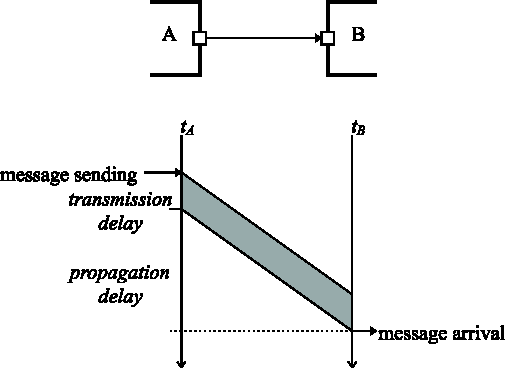
\includegraphics[width=4.301in, height=2.417in]{figures/usmanFig4}
\caption{Message transmission}
\label{fig:ch-overview:message-transm}
\end{center}
\end{figure}

The above model may not be suitable to model all protocols. In Token Ring
and FDDI, stations start to repeat bits before the whole frame arrives;
in other words, frames ``flow through'' the stations, being delayed only a few bits.
In such cases, the data rate modeling feature of {\opp} cannot be used.

If a message travels along a path, passing through successive links and
compound modules, the model behaves as if each module waited until the
last bit of the message arrives and only started its transmission
afterwards.
(Fig. \ref{fig:ch-overview:msg-multiple-ch}).

\begin{figure}[htbp]
\begin{center}
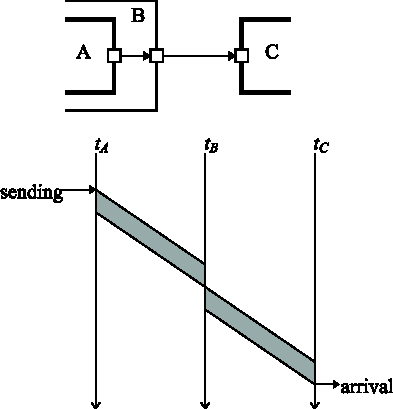
\includegraphics[width=3.330in, height=2.692in]{figures/usmanFig5}
\caption{Message sending over multiple channels}
\label{fig:ch-overview:msg-multiple-ch}
\end{center}
\end{figure}

Since the above effect is usually not the desired one, typically
you will want to assign data rate to only one connection in the
path.


\subsubsection{Multiple transmissions on links}

If a data rate\index{data rate} is specified for a connection, a message
will have a certain nonzero transmission time\index{transmission
  time}, depending on the length of the connection. This implies that
a message that is passsing through an output gate, ``reserves'' the gate
for a given period (``it is being transmitted'').

\begin{figure}[htbp]
  \begin{center}
    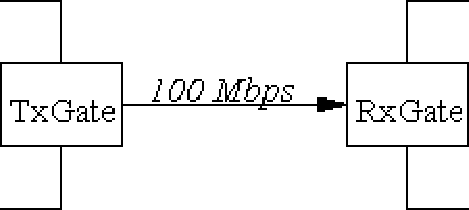
\includegraphics[width=2.315in, height=1.015in]{figures/usmanFig9}
    \caption{Connection with a data rate}
    \label{fig:ch-simple-modules:conn-w-data-rate}
  \end{center}
\end{figure}

While a message is under transmission, other messages have to wait
until the transmission is completed. The module sends another message while the
gate is busy, a runtime error will be thrown.

The {\opp} class library provides functions to check
whether a certain output gate is transmitting and find out when when
it finishes transmission.

If the connection with a data rate is not directly connected
to the simple module's output gate but is the second
one in the path, you have to check the second gate's busy
condition\index{gate!busy condition}.

\begin{note}
   In \opp versions prior to 4.0, sending on a busy gate was permitted, and
   messages got implicitly queued up. The behaviour of the simulation kernel
   was changed because in practice, sending on a busy gate was more often result
   of a programming error than calculated behaviour.
\end{note}


\subsubsection{Implementation of message sending}

Message sending is implemented like this: the arrival time\index{arrival time}
and the bit error\index{bit error} flag of a message are calculated right inside
the \fname{send()} call, then the message gets inserted into the FES\index{FES}
with the calculated arrival time. The message does \textit{not} get scheduled
individually for each link. This implementation was chosen because of its
run-time efficiency.

\begin{note}
   The consequence of this implementation is that any change in the
   channel's parameters (delay, bit rate, bit error rate) will only affect
   messages \textit{sent} after the change. Messages already under way will not
   be influenced by the change.

   This is not a huge problem in practice, but if it is important to model
   channels with changing parameters, the solution is to insert simple modules
   into the path to ensure strict scheduling.
\end{note}


\subsubsection{The approach of some other simulators}

Note that some simulators (e.g. OPNET) assign \textit{packet queues}
to input gates (ports), and messages sent are buffered at the
destination module (or the remote end of the link) until they are
received by the destination module. With that approach, events and
messages are separate entities, that is, a \textit{send} operation
includes placing the message in the packet queue \textit{and} scheduling
an event, which signals the arrival of the packet. In some implementations,
output gates also have packet queues where packets will be buffered until
the channel is ready (available for transmission).

{\opp} gates\index{gate} don't have associated queues. The place
where sent but not yet received messages are buffered in the
FES\index{FES}.  {\opp}'s approach is potentially faster
than the solution mentioned above because it doesn't have the
enqueue/dequeue overhead and also spares an event creation. The
drawback is, that changes to channel parameters do not take effect
immediately.

In {\opp} one can implement \textit{point-to-point transmitter} modules
with packet queues if needed. For example, the INET Framework
follows this approach.








\subsection{Broadcasts and retransmissions}

When you implement broadcasts or retransmissions, two frequently
occurring tasks in protocol simulation, you might feel tempted
to use the same message in multiple \fname{send()} operations.
Do not do it -- you cannot send the same message object multiple times.
The solution in such cases is duplicating the message.

\subsubsection{Broadcasting messages}

In your model, you may need to broadcast a message to several destinations.
Broadcast can be implemented in a simple module by sending out copies
of the same message, for example on every gate of a gate vector.
As described above, you cannot use the same message pointer for
in all \fname{send()} calls -- what you have to do instead is
create copies (duplicates) of the message object and send them.

Example:

\begin{verbatim}
for (int i=0; i<n; i++)
{
    cMessage *copy = (cMessage *) msg->dup();
    send(copy, "out", i);
}
delete msg;
\end{verbatim}

You might have noticed that copying the message for the last gate is
redundant (we could send out the original message),
so it can be optimized out like this:

\begin{verbatim}
for (int i=0; i<n-1; i++)   // note n-1 instead of n
{
    cMessage *copy = (cMessage *) msg->dup();
    send(copy, "out", i);
}
send(msg, "out", n-1);  // send original on last gate
\end{verbatim}


\subsubsection{Retransmissions}

Many communication protocols involve retransmissions of packets (frames).
When implementing retransmissions, you cannot just hold a pointer
to the same message object and send it again and again -- you'd get
the \textit{not owner of message} error on the first resend.

Instead, whenever it comes to (re)transmission, you should create and
send copies of the message, and retain the original.
When you are sure there will not be any more retransmission,
you can delete the original message.

Creating and sending a copy:

\begin{verbatim}
// (re)transmit packet:
cMessage *copy = (cMessage *) packet->dup();
send(copy, "out");
\end{verbatim}

and finally (when no more retransmissions will occur):

\begin{verbatim}
delete packet;
\end{verbatim}


\subsubsection{Why?}

A message is like any real world object -- it cannot be at two places
at the same time. Once you've sent it, the message object
no longer belongs to the module: it is taken over by the simulation kernel,
and will eventually be delivered to the destination module.
The sender module should not even refer to its pointer any more.
Once the message arrived in the destination module, that module
will have full authority over it -- it can send it on,
destroy it immediately, or store it for further handling.
The same applies to messages that have been scheduled -- they
belong to the simulation kernel until they are delivered back to
the module.

To enforce the rules above, all message sending functions
check that you actually own the message you are about to send.
If the message is with another module, it is currently scheduled or
in a queue etc., you'll get a runtime error: \textit{not owner of message}.
  \footnote{The feature does not increase runtime overhead significantly, because
  it uses the object ownership\index{ownership} management (described in
  Section \ref{sec:ch-sim-lib:ownership-management});
  it merely checks that the owner of the message is the module that
  wants to send it.}



\subsection{Delayed sending}

It is often needed to model a delay (processing time, etc.) immediately
followed by message sending. In {\opp}, it is possible to implement
it like this:

\begin{verbatim}
wait( someDelay );
send( msg, "outgate" );
\end{verbatim}


If the module needs to react to messages that arrive during the delay,
\fname{wait()} cannot be used and the timer mechanism described in
Section \ref{sec:ch-simple-modules:self-messages}, ``Self-messages'', would
need to be employed.


There is also a more straightforward method than those mentioned above:
delayed sending\index{delayed sending}. Delayed sending can be achieved
by using one of these functions:

\begin{verbatim}
sendDelayed(cMessage *msg, double delay, const char *gateName, int index);
sendDelayed(cMessage *msg, double delay, int gateId);
sendDelayed(cMessage *msg, double delay, cGate *gate);
\end{verbatim}

The arguments are the same as for \fname{send()}, except for the extra \textit{delay}
parameter. The effect of the function is the same as if the module
had kept the message for the delay interval and sent it afterwards.
That is, the sending time of the message will be the current
simulation time (time at the \fname{sendDelayed()} call) plus the delay.
The delay value must be non-negative.

Example:

\begin{verbatim}
sendDelayed(msg, 0.005, "outGate");
\end{verbatim}



\subsection{Direct message sending}

Sometimes it is necessary or convenient to ignore gates/connections
and send a message directly to a remote destination module. The \fname{sendDirect()}
function does that:

\begin{verbatim}
sendDirect(cMessage *msg, double delay, cModule *mod, int gateId)
sendDirect(cMessage *msg, double delay, cModule *mod, const char *gateName, int index=-1)
sendDirect(cMessage *msg, double delay, cGate *gate)
\end{verbatim}

In addition to the message and a delay, it also takes the destination module
and gate. The gate should be an \textit{input} gate and should not be connected.
In other words, the module needs dedicated gates for receiving via \ttt{sendDirect()}.
(Note: For leaving a gate unconnected in a compound module, you'll need to specify
\ttt{connections nocheck:} instead of plain \ttt{connections:} in the NED file.)

An example:

\begin{verbatim}
cModule *destinationModule = getParentModule()->getSubmodule("node2");
double delay = truncnormal(0.005, 0.0001);
sendDirect(new cMessage("packet"), delay, destinationModule, "inputGate");
\end{verbatim}

At the destination module, there is no difference between messages received
directly and those received over connections.



\subsection{Receiving messages}

\textbf{With activity() only!} The message receiving functions can
only be used in the \fname{activity()} function,
\fname{handleMessage()} gets received messages in its argument list.

Messages are received using the \fname{receive()} function.
\fname{receive()} is a member of \cclass{cSimpleModule}.

\begin{verbatim}
cMessage *msg = receive();
\end{verbatim}

The \fname{receive()} function accepts an optional \textit{timeout}
parameter\index{receive!timeout}. (This is a \textit{delta}, not an
absolute simulation time.) If an appropriate message doesn't arrive
within the timeout period, the function returns a NULL pointer.
    \footnote{Putaside-queue and the functions \ttt{receiveOn()},
    \ttt{receiveNew()}, and \ttt{receiveNewOn()} were deprecated
    in {\opp} 2.3 and removed in {\opp} 3.0.}

\begin{verbatim}
simtime_t timeout = 3.0;
cMessage *msg = receive( timeout );

if (msg==NULL)
{
    ...   // handle timeout
}
else
{
    ...  // process message
}
\end{verbatim}



\subsection{The wait() function}

\textbf{With activity() only!} The \fname{wait()} function's implementation
contains a \fname{receive()} call which cannot be used in \fname{handleMessage()}.

The \fname{wait()} function suspends the execution of the module for
a given amount of simulation time (a \textit{delta}).

\begin{verbatim}
wait(delay);
\end{verbatim}

In other simulation software, \fname{wait()} is often called \textit{hold}.
Internally, the \fname{wait()} function is implemented by a
\fname{scheduleAt()} followed by a \fname{receive()}.
The \fname{wait()} function is very convenient in modules that do not need
to be prepared for arriving messages, for example message generators.
An example:

\begin{verbatim}
for (;;)
{
  // wait for a (potentially random amount of) time, specified
  // in the interArrivalTime volatile module parameter
  wait(par("interArrivalTime").doubleValue());

  // generate and send message
  ...
}
\end{verbatim}

It is a runtime error if a message arrives during the wait interval.
If you expect messages to arrive during the wait period, you can
use the \fname{waitAndEnqueue()} function. It takes a pointer to a queue object
(of class \cclass{cQueue}, described in chapter \ref{cha:the-simulation-library})
in addition to the wait interval. Messages that arrive during the
wait interval will be accumulated in the queue, so you can
process them after the \fname{waitAndEnqueue()} call returned.

\begin{verbatim}
cQueue queue("queue");
...
waitAndEnqueue(waitTime, &queue);
if (!queue.empty())
{
  // process messages arrived during wait interval
  ...
}
\end{verbatim}


\subsection{Modeling events using self-messages}
\label{sec:ch-simple-modules:self-messages}

In most simulation models it is necessary to implement timers,
or schedule events that occur at some point in the future.
For example, when a packet is sent by a communications protocol model,
it has to schedule an event that would occur when a timeout expires,
because it will have to resent the packet then.
As another example, suppose you want to write a model of a server which
processes jobs from a queue. Whenever it begins processing
a job, the server model will want to schedule an event to occur
when the job finishes processing, so that it can begin processing
the next job.

In {\opp} you solve such tasks by letting the simple module
send a message to itself; the message would be delivered
to the simple module at a later point of time. Messages used
this way are called self-messages\index{self-message}.
Self-messages are used to model events which occur within the module.

\subsubsection{Scheduling an event}

The module can send a message to itself using the \fname{scheduleAt()} function.
\fname{scheduleAt()} accepts an \textit{absolute} simulation time,
usually calculated as \fname{simTime()}+\textit{delta}:

\begin{verbatim}
scheduleAt(absoluteTime, msg);
scheduleAt(simtime()+delta, msg);
\end{verbatim}

Self-messages are delivered to the module in the same way as other
messages (via the usual receive calls or \fname{handleMessage()});
the module may call the \fname{isSelfMessage()} member of any received
message to determine if it is a self-message.

As an example, here's how you could implement your own \fname{wait()}
function in an \fname{activity()} simple module, if the simulation kernel
didn't provide it already:

%
%TBD
%This looks like a pointless thing to do... Is there no better example?
%The kernel DOES after all, have a Wait() function built in...
%Of course, this is low priority.
%Gabor
%

\begin{verbatim}
cMessage *msg = new cMessage();
scheduleAt(simtime()+waitTime, msg);
cMessage *recvd = receive();
if (recvd!=msg)
   // hmm, some other event occurred meanwhile: error!
...
\end{verbatim}

You can determine if a message is currently in the FES\index{FES}
by calling its \fname{isScheduled()} member:

\begin{verbatim}
if (msg->isScheduled())
  // currently scheduled
else
  // not scheduled
\end{verbatim}


\subsubsection{Re-scheduling an event}

If you want to reschedule an event which is currently scheduled to a different
simulation time, first you have to cancel it using \fname{cancelEvent()}.


\subsubsection{Cancelling an event}

Scheduled self-messages can be cancelled\index{self-message!cancelling}
\index{message!cancelling} (removed from the FES\index{FES}).
This is particularly useful because self-messages are often used
to model timers.

\begin{verbatim}
cancelEvent( msg );
\end{verbatim}

The \fname{cancelEvent()} function takes a pointer to the message to
be cancelled, and also returns the same pointer. After having it
cancelled, you may delete the message or reuse it in the next
\fname{scheduleAt()} calls. \fname{cancelEvent()} gives an error if
the message is not in the FES\index{FES}.


\subsubsection{Implementing timers}

The following example shows how to implement timers:

\begin{verbatim}
cMessage *timeoutEvent = new cMessage("timeout");

scheduleAt(simTime()+10.0, timeoutEvent);
//...

cMessage *msg = receive();
if (msg == timeoutEvent)
{
  // timeout expired
}
else
{
  // other message has arrived, timer can be cancelled now:
  delete cancelEvent(timeoutEvent);
}
\end{verbatim}





\subsection{Stopping the simulation}

\subsubsection{Normal termination}

You can finish the simulation with the \fname{endSimulation()} function:

\begin{verbatim}
endSimulation();
\end{verbatim}

\fname{endSimulation()} is rarely needed in practice because you
can specify simulation time and CPU time limits\index{simulation time limits}
in the ini file (see later).

\subsubsection{Stopping on errors}

If you want your simulation to stop if it detects an error condition,
you can call the \fname{error()} member function of \cclass{cModule}.
Its argument list is similar to \fname{printf()}:

\begin{verbatim}
if (windowSize<1)
  error("Invalid window size %d; must be >=1", windowSize);
\end{verbatim}

Do not include a newline (``{\textbackslash}n'') or punctuation (period
or exclamation mark) in the error text; it will be added by {\opp}.





\section{Accessing module parameters}
\label{ch:simple-modules:parameters}

Module parameters declared in NED files are represented with the \cclass{cPar}
class at runtime, and be accessed\index{module!accessing parameters}
by calling the \fname{par()} member function of \cclass{cModule}:

\begin{verbatim}
cPar& delayPar = par("delay");
\end{verbatim}

\cclass{cPar}'s value can be read with methods that correspond to
the parameter's NED type: \fname{boolValue()}, \fname{longValue()},
\fname{doubleValue()}, \fname{stringValue()}, \fname{stdstringValue()},
\fname{xmlValue()}.
There are also overloaded type cast operators for the corresponding types
(\ttt{bool}; integer types including \ttt{int}, \ttt{long}, etc;
\ttt{double}; \ttt{const char *}; \ttt{cXMLElement *}).

\begin{verbatim}
long numJobs = par("numJobs").longValue();
double processingDelay = par("processingDelay"); // using operator double()
\end{verbatim}

Note that \cclass{cPar} has two methods for returning string value:
\fname{stringValue()} which returns \ttt{const char *}, and
\fname{stdstringValue()} which returns \ttt{std::string}.
For volatile parameters, only \fname{stdstringValue()} may be used,
but otherwise the two are interchangeable.

If you use the \ttt{par("foo")} parameter in expressions (such as
\ttt{4*par("foo")+2}), the C++ compiler may be unable to decide
between overloaded operators and report ambiguity. In that case
you have to clarify by adding either an explicit cast
(\ttt{(double)par("foo")} or \ttt{(long)par("foo")}) or use
the \ttt{doubleValue()} or \ttt{longValue()} methods.


\subsection{Volatile and non-volatile parameters}

A parameter can be declared \ttt{volatile} in the NED file. The \ttt{volatile}
modifier indicates that a parameter is re-read every time a value is needed
during simulation. Volatile parameters typically are used for things like
random packet generation interval, and get values like \ttt{exponential(1.0)}
(numbers drawn from the exponential distribution with mean 1.0).

In contrast, non-volatile NED parameters are constants, and reading their
values multiple times is guaranteed to yield the same value. When a non-volatile
parameter is assigned a random value like \ttt{exponential(1.0)}, it gets
evaluated once at the beginning of the simulation and replaced with the result,
so all reads will get same (randomly generated) value.

The typical usage for non-volatile parameters is to read them in the
\fname{initialize()} method of the module class, and store the values
in class variables for easy access later:

\begin{verbatim}
class Source : public cSimpleModule
{
  protected:
    long numJobs;
    virtual void initialize();
    ...
};

void Source::initialize()
{
    numJobs = par("numJobs");
    ...
}
\end{verbatim}

\ttt{volatile} parameters need to be re-read every time the value is needed.
For example, a parameter that represents a random packet generation interval
may be used like this:

\begin{verbatim}
void Source::handleMessage(cMessage *msg)
{
    ...
    scheduleAt(simTime() + par("interval").doubleValue(), timerMsg);
    ...
}
\end{verbatim}

This code looks up the the parameter by name every time. This lookup
can be spared by storing the parameter object's pointer in a class variable,
resulting in the following code:

\begin{verbatim}
class Source : public cSimpleModule
{
  protected:
    cPar *intervalp;
    virtual void initialize();
    virtual void handleMessage(cMessage *msg);
    ...
};

void Source::initialize()
{
    intervalp = &par("interval");
    ...
}

void Source::handleMessage(cMessage *msg)
{
    ...
    scheduleAt(simTime() + intervalp->doubleValue(), timerMsg);
    ...
}
\end{verbatim}


\subsection{Changing a parameter's value}

Parameter values can be changed from the program, during execution.
This is rarely needed, but may be useful for some scenarios.

\begin{note}
    The parameter's type cannot be changed at runtime -- it must
    remain the type declared in the NED file. It is also not possible
    to add or remove module parameters at runtime.
\end{note}

The methods to set the parameter value are \fname{setBoolValue()},
\fname{setLongValue()}, \fname{setStringValue()},
\fname{setDoubleValue()}, \fname{setXMLValue()}. There are also
overloaded assignment operators for various types including \ttt{bool},
\ttt{int}, \ttt{long}, \ttt{double}, \ttt{const char *}, and
\ttt{cXMLElement *}.

To let a module get notified about parameter changes, override
its \fname{handleParameterChange()} method, see
\ref{sec:handleParameterChange}.


\subsection{Further cPar methods}

The parameter's name and type are returned by the \fname{getName()} and
\fname{getType()} methods. The latter returns a value from an enum,
which can be converted to a readable string with the \fname{getTypeName()}
static method. The enum values are \ttt{BOOL}, \ttt{DOUBLE}, \ttt{LONG},
\ttt{STRING} and \ttt{XML}; and since the enum is an inner type,
they usually have to be qualified with \ttt{cPar::}.

\fname{isVolatile()} returns whether the parameter was declared volatile
in the NED file. \fname{isNumeric()} returns true if the parameter
type is double or long.

The \fname{str()} method returns the parameter's value in a string form.
If the parameter contains an expression, then the string representation
of the expression gets returned.

An example usage of the above methods:

\begin{verbatim}
int n = getNumParams();
for (int i=0; i<n; i++)
{
    cPar& p = par(i);
    ev << "parameter: " << p.getName() << "\n";
    ev << "  type:" << cPar::getTypeName(p.getType()) << "\n";
    ev << "  contains:" << p.str() << "\n";
}
\end{verbatim}

The NED properties of a parameter can be accessed with the \fname{getProperties()}
method that returns a pointer to the \cclass{cProperties} object that stores
the properties of this parameter. Specifically, \fname{getUnit()} returns
the physical unit associated with the parameter (\ttt{@unit} property in NED).

Further \cclass{cPar} methods and related classes like \cclass{cExpression} and
\cclass{cDynamicExpression} are used by the NED infrastructure to set up and
assign parameters. They are documented in the \tbf{API Reference}, but
they are normally of little interest for users.


\subsection{Emulating parameter arrays}

As of version 4.0, {\opp} does not support parameter arrays,
but in practice they can be emulated using string parameters.
One can assign the parameter a string which contains all values
in a textual form (for example, \ttt{"0 1.234 3.95 5.467"}), then
parse this string in the simple module.

The \cclass{cStringTokenizer} class can be quite useful for this
purpose. The constructor accepts a string, which it regards as
a sequence of tokens (words) separated by delimiter characters
(by default, spaces). Then you can either enumerate the tokens
and process them one by one (\fname{hasMoreTokens()}, \fname{nextToken()}),
or use one of the \cclass{cStringTokenizer} convenience methods to convert
them into a vector of strings (\fname{asVector()}), integers (\fname{asIntVector()}),
or \ttt{double}s (\fname{asDoubleVector()}).

The latter methods can be used like this:

\begin{verbatim}
const char *str = "aa bb cc";
std::vector<std::string> v = cStringTokenizer().asVector();

const char *str = "34 42 13 46 72 41";
std::vector<int> v = cStringTokenizer().asIntVector();

const char *str = "0.4311 0.7402 0.7134";
std::vector<double> v = cStringTokenizer().asDoubleVector();
\end{verbatim}

The following example processes the string by enumerating the tokens:

\begin{verbatim}
const char *str = "3.25 1.83 34 X 19.8"; // input

std::vector<double> result;
cStringTokenizer tokenizer(str);
while (tokenizer.hasMoreTokens())
{
    const char *token = tokenizer.nextToken();
    if (strcmp(token, "X")==0)
        result.push_back(DEFAULT_VALUE);
    else
        result.push_back(atof(token));
}
\end{verbatim}



\section{Accessing gates and connections}
\label{ch:simple-modules:gates}

\subsection{Gate objects}


Module gates\index{gate} are \cclass{cGate} objects. Gate objects
know whether, and to which gate they are connected. They can also be
queried on the parameters of the link (delay, data rate, etc.)

The \fname{gate()} member function of \cclass{cModule} returns a
pointer to a \cclass{cGate} object, and an overloaded form of the
function lets you access elements of a vector gate:

\begin{verbatim}
cGate *outgate = gate("out");
cGate *outvec5gate = gate("outvec",5);
\end{verbatim}

For gate vectors\index{gate!vector}, the first form returns the first gate in the
vector (at index 0).

The \fname{isVector()} member function can be used to determine if a
gate belongs to a gate vector or not.

Given a gate pointer, you can use the \fname{size()} and
\fname{getIndex()} member functions of \cclass{cGate} to determine the
size of the gate vector\index{gate!vector size} and the
index\index{gate!vector index} of the gate within the vector:

\begin{verbatim}
int size2 = outvec5gate->size(); // --> size of outvec[]
int index = outvec5gate->getIndex(); // --> 5 (it is gate 5 in the vector)
\end{verbatim}

Instead of \ttt{gate->size()}, you can also call the \fname{gateSize()}
method of \cclass{cModule}, which does the same:

\begin{verbatim}
int size2 = gateSize("out");
\end{verbatim}

For non-vector gates, \fname{size()} returns 1 and \fname{getIndex()} returns 0.

Zero-size gate vectors are represented with a placeholder gate whose
\fname{size()} method returns zero and cannot be connected.

The \fname{getType()} member function returns a character, 'I' for input
gates and 'O' for output gates:

\begin{verbatim}
char type = outgate->getType() // --> 'O'
\end{verbatim}


\subsubsection{Gate IDs}

Module gates (input and output, single and vector) are stored in an
array within their modules. The gate's position in the array is called
the \textit{gate ID}. The gate ID\index{gate!id} is returned by the \fname{getId()}
member function:

\begin{verbatim}
int id = outgate->getId();
\end{verbatim}

For a module with input gates \ttt{fromApp} and \ttt{in[3]} and output gates
of \ttt{toApp} and \ttt{status}, the array may look like this:

\begin{longtable}{|c|c|c|}
\hline
% ROW 1
\tabheadcol
\textbf{ID} & \textbf{dir} & \textbf{name[index]}\\\hline
% ROW 2
0 & \textit{input} & \ttt{fromApp} \\\hline
% ROW 3
1 & \textit{output} & \ttt{toApp} \\\hline
% ROW 4
2 & \multicolumn{2}{c|}{\textit{empty}}\\\hline
% ROW 5
3 & \textit{input} & \ttt{in[0]}\\\hline
% ROW 6
4 & \textit{input} & \ttt{in[1]}\\\hline
% ROW 7
5 & \textit{input} & \ttt{in[2]}\\\hline
% ROW 8
6 & \textit{output} & \ttt{status}\\\hline
\end{longtable}

The array may have empty slots. Gate vectors are guaranteed to
occupy contiguous IDs, thus it is legal to calculate the
ID of \textit{gate[k]} as \ttt{gate("gate",0).getId()+k}.

Message sending and receiving functions accept both gate names
and gate IDs; the functions using gate IDs are a bit faster.
Gate IDs do not change during execution, so it is often worth
retrieving them in advance and using them instead of gate names.

You can also obtain gate IDs with the \fname{findGate()}
member of \cclass{cModule}:

\begin{verbatim}
int id1 = findGate("out");
int id2 = findGate("outvect",5);
\end{verbatim}



\subsection{Connection parameters}

Connection attributes (propagation delay, transmission data rate,
bit error rate) are represented by the channel object, which
is available via the source gate of the connection.

\begin{verbatim}
cChannel *chan = outgate->getChannel();
\end{verbatim}

\cclass{cChannel} is a small base class. All interesting attributes are
part of its subclass \cclass{cDatarateChannel}, so you have to cast the pointer
before getting to the delay, error and data rate values.

\begin{verbatim}
cDatarateChannel *chan = check_and_cast<cDatarateChannel *>(outgate->getChannel());
double d = chan->getDelay();
double e = chan->getBitErrorRate();
double r = chan->getDatarate();
\end{verbatim}

You can also change the channel attributes with the corresponding
\ttt{setXXX()} functions. Note, however, that (as it was explained in
section \ref{ch:simple-modules:packet-transmission})
changes will not affect messages already sent, even if they have not
begun transmission yet.



\subsection{Transmission state}
\label{ch:simple-modules:cgate-transmission-state}

The \fname{isBusy()} member function returns whether the gate
is currently transmitting, and if so, the
\fname{getTransmissionFinishTime()} member function
returns the simulation time when the gate is going to finish
transmitting. (If the gate in not currently transmitting,
\fname{getTransmissionFinishTime()} returns the simulation time
when it finished its last transmission.)

The semantics have been described in section
\ref{ch:simple-modules:packet-transmission}.

An example:

\begin{verbatim}
cMessage *packet = new cMessage("DATA");
packet->setByteLength(1024);  // 1K

if (gate("TxGate")->isBusy()) // if gate is busy, wait until it
{                             // becomes free
  wait( gate("TxGate")->getTransmissionFinishTime() - simTime());
}
send( packet, "TxGate");
\end{verbatim}

If the connection with a data rate is not directly connected
to the simple module's output gate but is the second
one in the path, you have to check the second gate's busy
condition\index{gate!busy condition}. You could use the following
code:

\begin{verbatim}
if (gate("mygate")->getToGate()->isBusy())
  //...
\end{verbatim}

Note that if data rates change\index{data rate change} during the
simulation, the changes will affect only the messages that are
\textit{sent} after the change.



\subsection{Connectivity}

The \fname{isConnected()} member function returns whether
the gate is connected. If the gate is an output gate, the gate to
which it is connected is obtained by the \fname{getToGate()}
member function. For input gates, the function is
\fname{getFromGate()}.

%
% TBD figure
%

\begin{verbatim}
cGate *gate = gate("somegate");
if (gate->isConnected())
{
  cGate *othergate = (gate->getType()=='O') ?
                     gate->getToGate() : gate->getFromGate();

  ev << "gate is connected to: " << othergate->getFullPath() << endl;
}
else
{
  ev << "gate not connected" << endl;
}
\end{verbatim}


An alternative to \fname{isConnected()} is to check the return value
of \fname{getToGate()} or \fname{getFromGate()}. The following code is fully equivalent
to the one above:

\begin{verbatim}
cGate *gate = gate("somegate");
cGate *othergate = (gate->getType()=='O') ?
                   gate->getToGate() : gate->getFromGate();
if (othergate)
  ev << "gate is connected to: " << othergate->getFullPath() << endl;
else
  ev << "gate not connected" << endl;
\end{verbatim}

To find out to which simple module a given output
gate leads finally\index{gate!destination}, you would have to walk
along the path like this (the \fname{getOwnerModule()} member function
returns the module to which the gate belongs):

\begin{verbatim}
cGate *gate = gate("out");
while (gate->getToGate()!=NULL)
{
  gate = gate->getToGate();
}

cModule *destmod = gate->getOwnerModule();
\end{verbatim}


but luckily, there are two convenience functions which do that:
\fname{getSourceGate()} and
\fname{getDestinationGate()}.





\section{Walking the module hierarchy}
\label{ch:simple-modules:walking-module-hieararchy}

\subsubsection{Module vectors}


If a module is part of a module vector\index{module!vector}, the
\fname{getIndex()} and \fname{size()} member functions can be used to
query its index and the vector size:

\begin{verbatim}
ev << "This is module [" << module->getIndex() <<
      "] in a vector of size [" << module->size() << "].\n";
\end{verbatim}


\subsubsection{Module IDs}


Each module in the network has a unique ID that is returned by the
\fname{getId()} member function. The module ID\index{module!id} is used
internally by the simulation kernel to identify modules.

\begin{verbatim}
int myModuleId = getId();
\end{verbatim}

If you know the module ID, you can ask the simulation object
(a global variable) to get back the module pointer:

\begin{verbatim}
int id = 100;
cModule *mod = simulation.getModule( id );
\end{verbatim}


Module IDs are guaranteed to be unique, even when modules are
created and destroyed dynamically. That is, an ID which once
belonged to a module which was deleted is never issued to another
module later.


\subsubsection{Walking up and down the module hierarchy}


The surrounding compound module can be accessed by the
\fname{getParentModule()} member function:

\begin{verbatim}
cModule *parent = getParentModule();
\end{verbatim}

For example, the parameters of the parent module are accessed
like this:

\begin{verbatim}
double timeout = getParentModule()->par( "timeout" );
\end{verbatim}


\cclass{cModule}'s \fname{findSubmodule()} and \fname{getSubmodule()}
member functions make it possible to look up the module's submodules
by name\index{module!submodule!lookup} (or name+index if the submodule
is in a module vector). The first one returns the numeric module ID of
the submodule, and the latter returns the module pointer.  If the
submodule is not found, they return -1 or NULL, respectively.

\begin{verbatim}
int submodID = compoundmod->findSubmodule("child",5);
cModule *submod = compoundmod->getSubmodule("child",5);
\end{verbatim}


The \fname{getModuleByRelativePath()} member function can be used to find
a submodule nested deeper than one level below. For example,

\begin{verbatim}
compoundmod->getModuleByRelativePath("child[5].grandchild");
\end{verbatim}

would give the same results as

\begin{verbatim}
compoundmod->getSubmodule("child",5)->getSubmodule("grandchild");
\end{verbatim}

(Provided that \ttt{child[5]} does exist, because otherwise the second
version would crash with an access violation because of the NULL
pointer dereference.)


The \cclass{cSimulation}::\fname{getModuleByPath()} function is similar
to \cclass{cModule}'s \fname{moduleByRelative\-Path()} function, and it
starts the search at the top-level module.


\subsubsection{Iterating over submodules}


To access all modules within a compound module,
use \cclass{cSubModIterator}.

For example:

\begin{verbatim}
for (cSubModIterator iter(*getParentModule()); !iter.end(); iter++)
{
  ev << iter()->getFullName();
}
\end{verbatim}

(\fname{iter()} is pointer to the current module the iterator is at.)


The above method can also be used to iterate along a module
vector\index{module!vector!iteration}, since the \fname{getName()}
function returns the same for all modules:

\begin{verbatim}
for (cSubModIterator iter(*getParentModule()); !iter.end(); iter++)
{
  if (iter()->isName(getName())) // if iter() is in the same
                              // vector as this module
  {
    int itsIndex = iter()->getIndex();
    // do something to it
  }
}
\end{verbatim}


\subsubsection{Walking along links}


To determine the module at the other end of a connection, use
\cclass{cGate}'s \fname{getFromGate()}, \fname{getToGate()} and
\fname{getOwnerModule()} functions. For example:

\begin{verbatim}
cModule *neighbour = gate( "outputgate" )->getToGate()->getOwnerModule();
\end{verbatim}


For input gates, you would use \fname{getFromGate()} instead of \fname{getToGate()}.


\section{Direct method calls between modules}
\label{ch:simple-modules:direct-method-calls}
\index{method calls!between modules}

In some simulation models, there might be modules which are too
tightly coupled for message-based communication to be efficient.
In such cases, the solution might be calling one simple module's public
C++ methods from another module.

Simple modules are C++ classes, so normal C++ method calls will
work. Two issues need to be mentioned, however:

\begin{itemize}
  \item how to get a pointer to the object representing the module;
  \item how to let the simulation kernel know that a method call across modules
     is taking place.
\end{itemize}

Typically, the called module is in the same compound module as the caller,
so the \fname{getParentModule()} and \fname{getSubmodule()} methods of
\cclass{cModule} can be used to get a \ttt{cModule*} pointer to the
called module. (Further ways to obtain the pointer are described
in the section \ref{ch:simple-modules:walking-module-hieararchy}.)
The \ttt{cModule*} pointer then has to be cast to the actual C++ class
of the module, so that its methods become visible.

This makes the following code:

\begin{verbatim}
cModule *calleeModule = getParentModule()->getSubmodule("callee");
Callee *callee = check_and_cast<Callee *>(calleeModule);
callee->doSomething();
\end{verbatim}

The \fname{check\_and\_cast<>()} template function on the second line
is part of {\opp}. It does a standard C++ \ttt{dynamic\_cast},
and checks the result: if it is NULL, \ttt{check\_and\_cast} raises an {\opp} error.
Using \ttt{check\_and\_cast} saves you from writing error checking
code: if \ttt{calleeModule} from the first line is NULL because
the submodule named \ttt{"callee"} was not found, or if that
module is actually not of type \ttt{Callee}, an error gets thrown
from \ttt{check\_and\_cast}.

The second issue is how to let the simulation kernel know that
a method call across modules is taking place. Why is this necessary
in the first place? First, the simulation kernel always has to know which
module's code is currently executing, in order to several internal
mechanisms to work correctly. (One such mechanism is ownership handling.)
Second, the Tkenv simulation GUI can animate method calls,
but to be able to do that, it has to know about them.

The solution is to add the \ttt{Enter\_Method()} or \ttt{Enter\_Method\_Silent()}
macro at the top of the methods that may be invoked from other
modules. These calls perform context switching, and, in case of
\ttt{Enter\_Method()}, notify the simulation GUI so that animation
of the method call can take place. \ttt{Enter\_Method\_Silent()}
does not animate the call. \ttt{Enter\_Method()} expects a
\ttt{printf()}-like argument list -- the resulting string will
be displayed during animation.

\begin{verbatim}
void Callee::doSomething()
{
    Enter_Method("doSomething()");
    ...
}
\end{verbatim}



\section{Dynamic module creation}
\label{ch:simple-modules:dynamic-module-creation}
\index{module!dynamic creation}

\subsection{When do you need dynamic module creation}

In some situations you need to dynamically create and maybe destroy
modules. For example, when simulating a mobile network,
you may create a new module whenever a new user enters
the simulated area, and dispose of them when they leave the area.

As another example, when implementing a server or a transport
protocol, it might be convenient to dymically create modules
to serve new connections, and dispose of them when the connection
is closed. (You would write a manager module that receives connection
requests and creates a module for each connection.
The Dyna example simulation does something like this.)

Both simple and compound modules can be created dynamically.
If you create a compound module, all its submodules will be created
recursively.

It is often convenient to use direct message sending with dynamically
created modules.

Once created and started, dynamic modules aren't any different from
``static'' modules; for example, one could also delete static modules
during simulation (though it is rarely useful.)


\subsection{Overview}


To understand how dynamic module creation works, you have to know a
bit about how normally {\opp} instantiates modules. Each module type
(class) has a corresponding factory object of the class
\cclass{cModuleType}. This object is created under the hood by the
\fmac{Define\_Module()} macro, and it has a factory
function\index{factory function} which can instantiate the module
class (this function basically only consists of a \ttt{return new
\textit{module-class}(...)} statement).

The \cclass{cModuleType} object can be looked up by its name
string (which is the same as the module class name). Once you have its
pointer, it is possible to call its factory method and create an
instance of the corresponding module class -- without having to
include the C++ header file containing module's class declaration
into your source file.

The \cclass{cModuleType} object also knows what gates and
parameters the given module type has to have. (This info comes from
compiled NED code.)

Simple modules can be created in one step. For a compound module, the
situation is more complicated, because its internal structure
(submodules, connections) may depend on parameter values and gate
vector sizes. Thus, for compound modules it is generally required to
first create the module itself, second, set parameter values and gate
vector sizes, and then call the method that creates its submodules and
internal connections.

As you know already, simple modules with \fname{activity()} need a
starter message\index{starter messages}. For statically created
modules, this message is created automatically by {\opp}, but for
dynamically created modules, you have to do this explicitly by calling
the appropriate functions.

Calling \fname{initialize()} has to take place after insertion of the
starter messages, because the initializing code may insert new messages
into the FES\index{FES}, and these messages should be processed
\textit{after} the starter message.

%
% TBD
%


\subsection{Creating modules}

The first step, finding the factory object:

\begin{verbatim}
cModuleType *moduleType = cModuleType::get("WirelessNode");
\end{verbatim}


\subsubsection{Simplified form}

\cclass{cModuleType} has a
\ttt{createScheduleInit(const char *name, cModule *parentmod)}
convenience function to get a module up and running in one step.

\begin{verbatim}
mod = modtype->createScheduleInit("node",this);
\end{verbatim}

It does \fname{create()} + \fname{buildInside()} +
\fname[scheduleStart()]{scheduleStart(now)} + \fname{callInitialize()}.

This method can be used for both simple and compound modules.
Its applicability is somewhat limited, however:
because it does everything in one step, you do not have the chance to
set parameters or gate sizes, and to connect gates before
\fname{initialize()} is called.
(\fname{initialize()} expects all parameters and gates to
be in place and the network fully built when it is called.)
Because of the above limitation, this function is mainly useful
for creating basic simple modules.

%
% Example:
% TBD
%

\subsubsection{Expanded form}


If the previous simple form cannot be used. There are 5 steps:
\begin{enumerate}
  \item{find factory object}
  \item{create module}
  \item{set up parameters and gate sizes (if needed)}
  \item{call function that builds out submodules and finalizes the
    module}
  \item{call function that creates activation message(s) for the new
    simple getModule(s)}
\end{enumerate}
Each step (except for Step 3.) can be done with one line of code.



See the following example, where Step 3 is omitted:

\begin{verbatim}
// find factory object
cModuleType *moduleType = cModuleType::get("WirelessNode");

// create (possibly compound) module and build its submodules (if any)
cModule *module = moduleType->create("node", this);
module->buildInside();

// create activation message
module->scheduleStart( simTime() );
\end{verbatim}

If you want to set up parameter values or gate vector sizes (Step 3.),
the code goes between the \fname{create()} and
\fname{buildInside()} calls:

\begin{verbatim}
// create
cModuleType *moduleType = cModuleType::get("WirelessNode");
cModule *module = moduleType->create("node", this);

// set up parameters and gate sizes before we set up its submodules
module->par("address") = ++lastAddress;
module->setGateSize("in", 3);
module->setGateSize("out", 3);

// create internals, and schedule it
module->buildInside();
module->scheduleStart(simTime());
\end{verbatim}


\subsection{Deleting modules}


To delete a module dynamically\index{module!dynamic deletion}:

\begin{verbatim}
module->deleteModule();
\end{verbatim}

If the module was a compound module, this involves recursively
destroying all its submodules. A simple module can also delete itself;
in this case, the \fname{deleteModule()} call does not return to the
caller.

Currently, you cannot safely delete a
compound\index{module!compound!deletion} module from a simple module
in it; you must delegate the job to a module outside the compound
module.


\subsection{Module deletion and finish()}

When you delete a module \textit{during simulation}, its \fname{finish()}
function is not called automatically (\fname{deleteModule()} doesn't do it.)
How the module was created doesn't play any role here:
\fname{finish()} gets called for \textit{all} modules -- at the end of the
simulation. If a module doesn't live that long, \fname{finish()} is not
invoked, but you can still manually invoke it.

You can use the \fname{callFinish()} function to arrange \fname{finish()}
to be called. It is usually not a good idea to invoke \fname{finish()}
directly. If you're deleting a compound module, \fname{callFinish()} will
recursively invoke \fname{finish()} for all submodules, and if you're deleting
a simple module from another module, \fname{callFinish()} will do the context
switch for the duration of the call.
  \footnote{The \fname{finish()} function is even made \ttt{protected}
  in \cclass{cSimpleModule}, in order to discourage its invocation from
  other modules.}

Example:

\begin{verbatim}
mod->callFinish();
mod->deleteModule();
\end{verbatim}


\subsection{Creating connections}
\index{connection!creating}

Connections can be created using \cclass{cGate}'s \fname{connectTo()}
method.
  \footnote{The earlier \fname{connect()} global functions that
  accepted two gates have been deprecated, and may be removed
  from further {\opp} releases.}
\fname{connectTo()} should be invoked on the source gate
of the connection, and expects the destination gate pointer as
an argument:

\begin{verbatim}
srcGate->connectTo(destGate);
\end{verbatim}

The \textit{source} and \textit{destination} words correspond
to the direction of the arrow in NED files.

As an example, we create two modules and connect them in both directions:

\begin{verbatim}
cModuleType *moduleType = cModuleType::get("TicToc");
cModule *a = modtype->createScheduleInit("a",this);
cModule *b = modtype->createScheduleInit("b",this);

a->gate("out")->connectTo(b->gate("in"));
b->gate("out")->connectTo(a->gate("in"));
\end{verbatim}

\fname{connectTo()} also accepts a channel object as an
additional, optional argument. Channels are subclassed from
\cclass{cChannel}. Almost always you'll want use an instance of
\cclass{cDatarateChannel} as channel -- this is the one that supports
delay\index{channel!delay}, bit error rate \index{channel!error}
and data rate\index{channel!datarate}. The channel object will
be owned by the source gate of the connection, and you cannot
reuse the same channel object with several connections.

\cclass{cDatarateChannel} has \fname{setDelay()}, \fname{setBitErrorRate()}
and \fname{setDatarate()} methods to set up the channel attributes.

An example that sets up a channel with a delay:

\begin{verbatim}
cDatarateChannel *channel = new cDatarateChannel("channel");
channel->setDelay(0.001);

a->gate("out")->connectTo(b->gate("in"), channel); // a,b are modules
\end{verbatim}


\subsection{Removing connections}
\index{connection!removing}

The \fname{disconnect()} method of \cclass{cGate} can be
used to remove connections. This method has to be invoked
on the \textit{source} side of the connection. It also destroys
the channel object associated with the connection, if one has been set.

\begin{verbatim}
srcGate->disconnect();
\end{verbatim}


%%% Local Variables:
%%% mode: latex
%%% TeX-master: "usman"
%%% End:
